\documentclass[12pt,a4paper]{article}
\usepackage {amsmath,amsthm}
\usepackage{geometry}
\usepackage{titlesec}
 \geometry{a4paper, total={170mm,257mm}, left=20mm, right=20mm, top=25mm, bottom=25mm}
%\usepackage{tabularx}
\usepackage{sectsty}
\usepackage{natbib}
\bibliographystyle{econ}
\usepackage[hidelinks]{hyperref}
\usepackage{multirow}
\usepackage{makecell}
\usepackage{adjustbox}
\usepackage{threeparttable}

%\usepackage[colorlinks=true, urlcolor=Blue]{hyperref}
%\usepackage{titling}
\sectionfont{\fontsize{14}{15}\selectfont}
\subsectionfont{\fontsize{13}{15}\selectfont}

\titleformat*{\section}{\LARGE\bfseries}
\titleformat*{\subsection}{\Large\bfseries}


\usepackage{caption}
\captionsetup{belowskip=12pt,aboveskip=0pt}

\makeatletter
\setlength{\@fptop}{0pt}
\makeatother


\usepackage[dvipsnames]{xcolor}

\newcommand{\link}[1]{{\color{blue}\href{#1}{#1}}}

%TRACKING TOOL FOR ARYA: 
\newcommand{\agt}[1]{{\color{OliveGreen}#1}}
\newcommand{\agst}[1]{{\color{OliveGreen}\sout{#1}}}

%TRACKING TOOL FOR ALEX: 
\newcommand{\aut}[1]{{\color{Red}#1}}
\newcommand{\aust}[1]{{\color{Red}\sout{#1}}}

%TRACKING TOOL FOR ARYA: 
\newcommand{\pmt}[1]{{\color{Blue}#1}}
\newcommand{\pmst}[1]{{\color{Blue}\sout{#1}}}


%\usepackage{cite}
\usepackage{booktabs}
\usepackage{float}
\usepackage{setspace}
\usepackage{placeins}
\usepackage[list=true]{subcaption}
\captionsetup[sub]{font=footnotesize}

\usepackage{graphicx}


\newtheorem{theorem}{Proposition}
\newtheorem{hypothesis}{Hypothesis}
	\def\hypothesisautorefname{Hypothesis}
\newtheorem{result}{Result}
	\def\resultautorefname{Result}
\def\sym#1{\ifmmode^{#1}\else\(^{#1}\)\fi}


\title{\Large Crying Wolf in the Lab\\}
\author{\large Arya Gaduh, Peter McGee, Alexander Ugarov*}
\begin{document}
\maketitle
\onehalfspacing
\begin{abstract}{ Abstract is here ----}


\vspace{10pt}
\begin{singlespace}

\noindent {\footnotesize{}Keywords: alarms, value of information, information economics, information design, --- }{\thispagestyle{empty}}
\end{singlespace}
\end{abstract}

\vspace{180pt}
\newpage
\normalsize

\section{Introduction}

The 2010 gas blowout on Deep Horizon oil rig has killed 11 workers and caused one of the largest oil spills in history. The death toll was possibly aggravated by switching off a general safety alarm because its sirens interfered with workers' sleep.\footnote{https://www.nytimes.com/2010/07/24/us/24hearings.html} This illustrates the trade-off between false-positive and false-negative test results with false-positive rates leading to higher false alarm costs and false-negative resulting in missed events. 

Many real-life situations involve choosing binary tests to discover and prevent a negative outcome. Most binary tests transform continuous signals about the likelihood of an adverse state into simple yes/no prediction. This transformation relies on choosing a threshold for positive classification. Holding a continuous signal constant, a decrease in probability of no alarm in an adverse state (false-negative rate) corresponds to an increase in probability of alarm in a non-adverse state (false-positive rate). This trade-off motivates multiple discussions in medical diagnostics, alarm systems and extreme weather alerts. Despite ubiquity of binary alarms, there is little empirical evidence on how users evaluate alarms with different false-positive and false-negative rates. 

In order to understand preferences over these trade-offs, we study the demand for information in the framework with a potential protection action. The subject, first, receives a signal about the probability of an adverse event. Then she decides to protect or not. This environment describes several practically important scenarios including extreme weather alerts, medical testing and safety alarms. 

Some recent studies observe that many people put non-zero value on information about ego-relevant beliefs or future utility even if it has no apparent effect on subsequent decisions (all the citations). These preferences is not the focus of our study and hence we use relatively low stakes and ego-neutral information. As a result, our findings might not apply to settings with changing identity beliefs or to settings with delayed resolution of uncertainty and large potential payoffs. 

We find that the value of information in our setup weakly correlates with the willingness-to-pay. First, subjects on average underreact to quality of the signal, resulting in overpaying for low-quality signal and underpaying for high-quaity signals. Second, subjects tend to overreact to false-negative rates when the prior probability is low and overreact to false-positive positive rates when priors are high. We show that this pattern is most consistent with failure to estimate the effect of frequencies of false-positive and false-negative outcomes on the costs of using the signal. Xu (2020) similarly finds that individuals(?) do not properly account for priors and often choose tests not affecting optimal decisions even then more instrumental tests are available.

Our work is one of a few experimental studies measuring demand for information used for decision-making (instrumental information). Previous experimental studies studies the demand for signals in the prediction game in which subjects have to choose an optimal state under uncertainty. The field experiment conducted by \citep{hoffman_how_2016} finds that the demand for information increases with initial uncertainty, but decreases with the signal's accuracy. However, the decrease in accuracy is more modest than expected for a Bayesian decision-maker resulting in subjects underpaying for high-quality signals. The laboratory experiment of \citet{ambuehl_belief_2018} finds that subjects tend to underreact to the accuracy of the binary signal about state of the world, but put a premium on completely certain signals. The paper of \citet{xu_revealed_2020} similarly employs a prediction game but varies priors on top of signal charasteristics. reducing prior uncertainty makes more signals non-instrumental in the sense that there should be no effect from a signal to optimal decisions.  She find that many subjects choose non-instrumental over instrumental signals which is consistent with

Our setup differs in two important aspects from \citep*{ambuehl_belief_2018, xu_revealed_2020}, because we study alerts and not prediction tasks. The subject faces a costly protection decision and not a prediction decision, resulting in three distinct payoffs: full payoff, full payoff minus protection costs and full payoff minus losses. It means that risk preferences affect the value of information and can change sensitivities to false-positive and false-negative rates. Our findings however are similar to prediction game findings. Consistent with \citet{ambuehl_belief_2018} we also find that subjects undervalue accurate signals, but we do not find a premium for certain signals.  And similar to \citet{xu_revealed_2020} we find that subjects do not properly account for interaction between prior probabilities and signal characteristics.

Due to its applicability for studying preferences over expectations, there is a larger stream of literature on the demand for non-instrumental information. \citet{eliaz_paying_2010} find that subjects are willing to pay for signals even when these signals are excessive for making optimal choices. Their design involves subjects choosing between two boxes with one box containing a prize of \$20. Most subjects pay just to know the probability of finding \$20 in box A even if this box is more likely to contain a prize in all the possible states. This finding is inconsistent with expected utility maximization but indicates instead having preferences for certainty before making choices.  Similar to this paper, \citet{masatlioglu_intrinsic_2017} also study preferences over information structures differing which differ in false-positive and false-negative rates but in their setup allows for a larger role of expectations. They find that for a positive potential outcome, most subjects prefer facing high false-negative rates rather than high false-positive rates. In other words, they tolerate uncertainty after negative signals better than uncertainty after positive signals. These preferences are salient: subjects require an average payment of 18-35 cents to switch to their least preferred information structure.

There is some mixed evidence that people update beliefs differently when these beliefs are ego-relevant or concern future gains and losses. \citet{eil_good_2011} find asymmetry in updating ego-relevant beliefs such as beauty and IQ. Subjects update more after receiving positive signals and do not update enough after negative signals. Additionally, subjects with high posterior ego-relevant beliefs are willing to pay to receive a more precise signals, but require a compensation for learning when their beliefs are low. In contrast, \citet{coutts_good_2019} does not find any updating asymmetry with respect to either ego-relevant beliefs or beliefs about future payoffs. 

Our paper is the first to measure value of information in the experimental setting of diagnostic tests or alarms. Previous work studies the use of alarms in context of medical testing, medical monitoring, safety alarms and extreme weather. Early literature on decision-making of medical professionals finds that doctors suffer from multiple biases when ordering testing, including  inaccurate posterior probability estimation due to availability heuristics, hindsight bias and regret \citep{bornstein_rationality_2001}. \citet{gigerenzer_helping_2007}find that very few mammologists understand mamogram results and tend to overestimate probability of cancer based on a positive result. Providing practitioners with natural frequencies instead of probabilities tends to reduce this bias.  

Patients' willingness-to-pay for medical tests is large and largely responsive to test accuracy \citep{liang_acceptability_2003, howard_does_2009, neumann_willingness--pay_2012}. But there are several apparent violations of rationality. First, users are willing to pay for tests having little or zero diagnostic value \citep{schwartz_enthusiasm_2004, neumann_willingness--pay_2012}. For example, \citet{schwartz_enthusiasm_2004} find that 73\% of Americans in their survey prefer a free full-body CT scan versus one thousand USD cash. However, medical professional do not recommend full-body CT scans for healthy people due to extreme likelihood of false-positive findings. Second, the framing of test accuracy seems to matter a lot. \citet{howard_does_2009} conduct a discrete-choice experiment to measure willingness-to-pay for the colorectal cancer screening. Their subjects agree to get 23 unnecessary colonoscopies in order to find one additional true cancer, but only 10.4 for reducing the number of cancers missed by one even though these descriptions are equivalent. Surprisingly, the perceived risk of cancer (prior) did not significantly affect the WTP in their study though the effect may come from its relatively low variation in the population.

This work also relates to the vast literature on demand for insurance and protection. Similar to our findings, several studies observe that the demand for insurance goes up after the recent experience with low-probabiity events. Field evidence indicates that people underinsure with respect to rare natural disasters (Friedl et al, 2014). \citet{laury_insurance_2009} find no under-insurance for low-probability events in the laboratory setting. One offered explanation \citep{volkman-wise_representativeness_2015} is that subjects overweight recent evidence leading to underinsurance when there were no negative events in the recent past and to overinsurance after the fact. It is consistent with underweighting prior probabilities relative to more recent signals. 

The bias we are finding is similar to the base-rate and signal neglect phenomenons. Psychology researchers \citet{hammerton_case_1973} and \citet{kahneman_psychology_1973} first observed that subjects underweighted prior probabilities (base rates) when calculating posteriors. This phenomenon had received the name of \textit{base-rate neglect}. Multiple studies in economics then confirmed \citep*{grether_testing_1992, holt_update_2009} this phenomenon in incentivized laboratory experiments. Most of these studies find that subjects also underweight signals on top of priors.  We observe both phenomenons in responses to our belief elicitation task, but the calculation of signals' values differs substantially from the calculation of posterior probabilities. While the calculation of posterior probabilities would require using a Bayes formula, signal's value depends only on products of prior probabilities. However, we observe that subjects underestimate the effect of priors compared to theoretical predictions for an expected-utility decision-maker.


\vspace{20pt}

\section{Model}
\vspace{10pt}
\bf Environment. \rm The model describes a decision-maker considering a purchase of threat-assessment information. Let $\omega \in \{0,1\}$ denote the state of world, where 1 corresponds to some adverse event happening with probability $\pi$. The decision-maker has a lower utility in the adverse state, but only if she does not take the protective action. Denote actions by $a\in\{0,1\}$ with 1 meaning taking the protective action. The protection technology is perfect: protected agents bear no losses but pay protection costs $c$ regardless of the state $\omega$. Decision-maker preferences are described by the utility function which depends on wealth $Y$, protective action $a$ and potential damage in the adverse state $\omega(1-a)$. Utility is separable in wealth, protection costs $c>0$ and potential loss in the adverse state $L>c$ \footnote{Separability condition does not impose additional restrictions on the utility function $U$ as long as the variation in wealth has limited range. More specifically, if $Y \in [Y_{min},Y_{max}]$ and $c<Y_{max}-Y_{min}, L<c+(Y_{max}-Y_{min})$, then the function $u(\cdot)$ can be constructed from segments of $U(\cdot,0,0), U(\cdot,1,0), U(\cdot,0,1)$.  While the resulting function $u(\cdot)$ is not necessarily monotonic, it is likely to be monotonic if protective actions and potential damages are relatively high.}:
\begin{equation}
U=U(Y,a,\omega(1-a))=u(Y-ac-\omega(1-a)L)
\end{equation}

The decision-maker can purchase a binary informative signal $s\in\{0,1\}$ about the state of the world before making a decision. Let $P_{ij}\equiv P(s=i|\omega=j)$ be the probability of a signal taking value $i$ conditional on the state of the world being $j$.  After receiving the signal, the decision-maker updates her belief on the likelihood of the bad state to $\mu(s)$. Unless specified otherwise, we assume that the decision-maker forms her posterior beliefs by using the Bayes rule. Hence the posterior belief equals:
\begin{equation}
\mu(s)= {\pi P_{s1} \over \pi P_{s1}+(1-\pi)P_{s0}}
\end{equation}

We also assume without loss of generality that a higher signal means a higher posterior probability of an adverse event $\mu(1)\geq\mu(0)$. Otherwise we can always re-label the signals.

\vspace{10pt}
\bf Preferences. \rm If there is no signal, the decision-maker protects if and only if it increases their expected utility:
\begin{equation}
EU_0=\max[u(Y-c),\pi u(Y-L)+(1-\pi) u(Y)]
\end{equation}
The signal can increase expected utility if the decision-maker reacts differently to positive and negative signals. Under these assumptions, her expected utility with a signal is:
\begin{equation}
EU_s=\pi P_{11}u(Y-c)+\pi P_{01}u(Y-L)+(1-\pi)P_{10}u(Y-c)+(1-\pi)P_{00}u(Y)
\end{equation}

We consider the maximum amount $b$ which the decision-maker is willing to pay for the signal. In our framework, it is a price paid with a signal such that a decision-maker is indifferent between having a signal and paying $b$ and not having a signal. Because the decision-maker can always ignore a useless signal, the signal's value is bounded from below by zero. Hence it equals to the maximum between zero and the solution to the following equation:
\begin{equation}
\begin{split}
P(s=1)u(Y-b-c)+\pi P_{01}u(Y-b-L)+(1-\pi)P_{00}u(Y-b)=\\=\max[u(Y-c),\pi u(Y-L)+(1-\pi) u(Y)] 
\end{split}
\end{equation}

The left-hand side expression of this equation is a strictly decreasing function of $b$. Additionally, for $b\rightarrow \infty$ the left-hand side is smaller than the right-hand side. It implies that the equation (5) above has a at most one positive solution.

Obviously, perfectly accurate signals always have positive value $b>0$ because the payoff distribution with the signal first-order stochastically dominates the distribution without the signal. If the decision-maker protects without a signal, a perfect signal reduces the protection costs and if she takes chances, then it reduces losses in the adverse outcome from $L$ to $c<L$.  However, it is harder to determine the value of the imperfect signal without imposing more restrictions on preferences as it requires weighing $u(Y-L)$ against $u(Y-c)$.


\vspace{10pt}
\bf Risk-neutral agent. \rm If the decision-maker is risk-neutral, the expression above collapses to:
$$b+P(s=1)c+\pi P_{01}L=\min[c,\pi L]$$

The signal's value is just:
\begin{equation}
b=\max[0,\min[c,\pi L]-P(s=1)c-\pi P_{01}L]
\end{equation}

We can express WTP $b$ as a function of priors, false-positive and false-negative rates. This is the equation we use in our empirical work:
\begin{equation}
b=\max[0,\min[c,\pi L]-\pi (1-P_{01})c-(1-\pi)P_{10}c-\pi P_{01}L]
\end{equation}

The sensitivity of (positive) value $b$ with respect to false-positive and false-negative rates is given by:
\begin{equation}
{db\over dP_{10}}=-(1-\pi)c
\end{equation}

\begin{equation}
{db\over dP_{10}}=-\pi(L-c)
\end{equation}
\vspace{10pt}

Both false-positive and false-negative rates decrease the (positive) signal's value. The effect is proportional to the adverse state probability for the false-negative rate and to the non-adverse state probability for the false-positive rates.

\vspace{10pt}
\bf Risk Aversion Effects. \rm In a more general expected utility framework, risk aversion can both increase and decrease the signal's value. More specifically, risk aversion decreases the value when the protection costs are low: 

\begin{theorem}
 If protection costs are low $c<\pi L$, then the strictly risk-averse decision-maker pays less than a risk-neutral one.
\end{theorem} 
\begin{proof}
See the Appendix.
\end{proof}
It is harder to make definite statements for lower risks or higher protection costs. For example, risk aversion increases value of a perfect signal as long as risk-averse decision-maker still chooses to not protect without a signal. This follows from the standard argument of increasing demand for insurance with risk aversion and the fact that the protection problem with a perfect signal is isomorphic to the insurance problem with deductible $c$. 

Next, we study the effect of false-positive and false-negative rates on the signal's value $b$. Assuming a differentiable utility function $u()$ we use implicit differentiation to derive sensitivities of WTP $b$ to false-positive and false-negative rates:

$${db\over dP_{10}}=-{(1-\pi)(u(Y-b)-u(Y-c-b))\over D(\pi, P_{01}, P_{10}, b)}$$
$${db\over dP_{01}}=-{\pi(u(Y-c-b)-u(Y-L-b))\over D(\pi, P_{01}, P_{10}, b)}$$

With the denominator equal to the expected marginal utility:
$$D(\pi, P_{01}, P_{10}, b)\equiv P(S=1)u'(Y-c-b)+\pi P_{01}u'(Y-L-b)+$$
$$+(1-\pi)P_{00}u'(Y-b)=E[MU]>0$$

It is clear that the signal's value decreases with false-positive and false-negative rates ${db\over dP_{10}},{db\over dP_{01}}<0$. We can also say a bit more about the sensitivity to false-negative rates:
\begin{theorem}
Risk-averse and imprudent decision-maker has higher sensitivity to false-negative rates as compared to a risk-neutral one.
\end{theorem} 
\begin{proof}
Use the mean value theorem to rewrite the sensitivity as:
$${db\over dP_{01}}=-{\pi u'(\zeta)(L-c)\over E[MU]},\zeta \in \left(Y-c-b, Y-L-b\right)$$
Now let $X$ denote a random payoff of the decision-maker with a signal. A risk-averse decision-maker puts a positive value on the signal only if its expected payoff is higher than the payoff with full protection: $EX>Y-c-b$. If a decision-maker is imprudent ($u'''<0$) then $E[MU]\equiv E[u'(X)]<u'(EX)$. Next, because $u'$ is a strictly increasing function and $EX>Y-c-b$: $u'(\zeta)>u'(Y-c-b)>u'(EX)$. Hence ${u'(\zeta)\over E[MU]}>1$ and ${db\over dP_{01}}<-\pi(L-c)$. 
\end{proof}


However, risk aversion can both increase and decrease subject's sensitivity to false-positive rates depending on the utility function curvature and signal's characteristics. Intuitively, an expected marginal utility of a strongly risk-averse subject with a bad signal can be lower than the average slope of the utility function between $Y-c-b$ and $Y-b$ reducing sensitivity to false-positive rates. It can also be higher if either the signal is good or the curvature is small. 

\vspace{20pt}

\section{Experimental Design}

In each session, subjects received a USD 5 show-up fee and were endowed with USD 25 that they might lose in the experiment. Subjects must then make a series of decisions in four sets of tasks: (i) Blind Protection; (ii) Informed Protection; (iii) Belief Elicitation; and (iv) Willingness to Pay Elicitation. To verify that subjects understand these tasks, they must answer a quiz before each task. If a subject gets any answer wrong, they read correct answers and explanations for each wrong answer. Additionally, subjects receive extra questions if they give wrong answers in a 5-question quiz given before the Informed Protection task. We do this because we consider Informed Protection as a first challenging task in the sequence which understanding is essential for the rest of the tasks. 
Each set of tasks has 6 rounds, for a total of 24 rounds. One of these rounds is selected at random as the payment round. A copy of the instruction is included in Appendix XX.

\bigskip
\noindent\textbf{Blind Protection (BP)}.\ \ \ In each BP round, subjects must decide whether to insure (or “protect”) against an adverse event (i.e., drawing a black ball from a box).  Subjects were informed of the prior probability of drawing a black ball before making their decision. The cost to protect is USD 5. If a black ball is drawn, an unprotected subject will lose USD 20. Subjects then played six rounds, where the probability of drawing a black ball was varied between XX and XX percent in each round. During the BP task, subjects did not receive any feedback on how that round would have been realized were it chosen as the payment round.

\bigskip
\noindent\textbf{Informed Protection (IP)}.\ \ \ For the IP task, subjects make a protection decision as in BP. However, before each decision, subjects are given a signal that was generated with varying degrees of inaccuracy. Following Coutts (2019), we present the signal-generation process using groups of ``gremlins'' that represent three types of signals: accurate (an honest gremlin), false positive (a black-swamp gremlin that always announces that the ball is black), and false negative (a white-swamp gremlin that always announces that the ball is white). Figure XX illustrates how the different gremlin types were presented to the subjects. Subjects knew the composition of the group from which the hint came from, but did not know which gremlin provided the hint. We vary the proportion of black balls in the box (prior probability of a black ball) and the composition of gremlins (signal quality) between rounds.  

\bigskip
\noindent\textbf{Belief Elicitation (BE)}.\ \ \ We use the BE task to elicit subjects’ beliefs about the likelihood of an adverse event and an adverse signal conditional on prior and signal characteristics in an incentive-compatible way. Similar to the IP task, subjects were informed of the prior probability of a black ball and the composition of the group of gremlins that would provide an additional signal. However, instead of asking subjects to make a protection decision, we asked them to estimate the probability of two events, to wit: (i) the ball is black ball when a randomly drawn gremlin says that it is white; (ii) the ball is black when a randomly drawn gremlin says that it is black.   

We follow the stochastic version of the Becker-DeGroot-Marshak mechanism developed by \citet{grether_testing_1992} and \citet{holt_update_2009} to elicit incentive-compatible responses: the subject submits their belief of the probability of the event $\mu \in [0,1]$. If this belief is above some uniform random number $r\in[0,1]$, they receive the payoff $x$ only if the stated event happens. Otherwise their payoff is determined by an independent lottery which pays $x$ with probability $r$ and 0 otherwise.\footnote{The benefit of this mechanism versus other probability elicitation mechanism (for example, quadratic scoring) is that reporting truthfully is a dominant strategy regardless of risk preferences \citep{karni_mechanism_2009-1}. The only requirements a subject needs to satisfy are probabilistic sophistication and dominance: they rank lotteries based on their probabilities only and prefer higher probabilities of higher payoffs.} To help subjects understand this complex mechanism, we prefaced our explanation of it with the fact that under this mechanism, truthful reporting of beliefs is the dominant strategy.

\bigskip
\noindent\textbf{Willingness to Pay Elicitation (WTPE)}.\ \ \ The WTPE task measures subjects' willingness to pay (WTP) for signals. Subjects know the prior probability of a black ball and the group composition of the gremlins that will determine signal quality.  We then ask subjects for their WTP to receive a hint from a randomly drawn gremlin. Subjects can choose a value from USD 0 to 5 with USD 50-cent increments. Their decisions are incentive compatible: if a WTPE round is selected as the payment round, a random price of a hint will be drawn. If that price exceeded the subjects’ WTP, they will play a BP round. Otherwise, the subject would pay for the hint and play an IP round.  After completing the WTPE task, subjects were asked a few demographic questions. The session concluded with the random selection and realization of the payment round, after which subjects were paid and dismissed.

The first three tasks were designed to provide measures of the different components of WTP described in Section XX and use them to examine the extent to which they explain subjects’ WTP measured in the WTPE task. We use the BP task both to measure subjects’ responses to the prior and their risk aversion. Next, we use the IP task to examine how signals affect protection decisions. Finally, we use the BE task as a measure of subjects’ ability to estimate the probability of a signal for a given quality and to perform Bayesian updating. To construct these measures, we presented our subjects with 6 different priors for the BP task, and 3 priors and 2 gremlin groupings for the IP, BE, and WTPE tasks. Table~ref{tab:treatments} XX shows the values of the different priors in our treatments, as well as the gremlin groupings (along with the associated false positive and false positive rates) that we used for the different tasks.

We conducted this experiment in the Behavioral Business Research Lab (BBRL) at the University of Arkansas between October and November 2021.  The experiment was implemented using Qualtrics. There were a total of 105 subjects. 84 percent of the subjects were university students and 41 percent were male.  About 60 percent of the subjects had taken at least one statistics course. On average, including the show-up fee, subjects received around USD 26 for a session lasting around 45 minutes.  



%%%%%%%%%%%%%%%%%%%%%%%%%%%%%%%%%%%%%%%%%%%%%%%%%%%%%%%%%%%%%%%%%%%%%%%%%%%%%%%%%%%%%%%%%%%%%%%%%%%%%%%%

\begin{table}[h!]
\caption{List of Treatments} \label{tab:treatments}
\begin{tabular}{l*{6}{c}}
\hline\hline
 & \multicolumn{3}{c} {Gremlins composition} & & \\
Prop. of black balls ($p$) & Honest & Black-eyed &White-eyed & FP rate &  FN rate\\
\hline
0.1, 0.2, 0.3, 0.5         &    2 & 0  &  0 & 0 & 0\\

0.1, 0.2, 0.3, 0.5         &    3 & 1  &  0 & 0.33 & 0  \\

0.1, 0.2, 0.3, 0.5          &    3 & 0  &  1 & 0 & 0.33 \\

0.1, 0.2, 0.3, 0.5           &    3 & 1  & 1 & 0.33 & 0.33\\

0.1, 0.2, 0.3, 0.5         &    5 & 1  & 0 & 0.2 & 0\\
0.1, 0.2, 0.3, 0.5         &    5 & 0  & 1 & 0 & 0.2    \\
0.1, 0.2, 0.3, 0.5         &    5 & 1 & 1  & 0.2 & 0.2  \\
\hline\hline
\end{tabular}


\end{table}

%%%%%%%%%%%%%%%%%%%%%%%%%%%%%%%%%%%%%%%%%%%%%%%%%%%%%%%%%%%%%%%%%%%%%%%%%%%%%%%%%%%%%%%%%%%%%%%%%%%%%%%%






\vspace{20pt}
\section{Results}\label{sec:results}
We begin with a brief overview of subject behavior in the different tasks. 

XXXX NEED TO REWRITE HERE XXXX

We follow that discussion with a regression analysis to explain subjects’ WTP for signals of different qualities. Our regression results suggest that subjects’ WTP deviated from those of a risk-neutral utility maximizing subject which was driven by their failure to fully account for signal quality when calculating their WTP. Furthermore, we find that these deviations remained after controlling for risk aversion or subjects’ ability to perform Bayesian updating. 

%The final subsection explored theories that are consistent with these observed behaviors.





\subsection{Overview: Are Subjects Bounded Rational?}


\textbf{Risk Aversion.}\ \ \ Subjects’ responses in the BP task are generally consistent with the expected utility framework. Figure~\ref{fig:ProtResponse} shows the probability of protection decision given prior probability of a black ball from the BP task. Subjects protected more with a higher probability of a negative outcome: only 13\% subjects protect when the probability of a black ball is 10\% in contrast to 70\% protecting when the probability is 30\%. 
%Moreover, the majority of subjects (54\%) have a probability threshold above which they always protect. About 30\% of subjects make at least one switch in which they protect for probability $P_1$ and do not protect for at least one probability $P_2>P_1$. 
About 30\% of subjects vacillated between protecting and not protecting; however, most of them (24 out of 39) vacillated only once, skipping a single increment of the presented probability scale, suggesting an inattention error.
Following \agt{XX ALEX: Any cite? XX}, we ``corrected'' these single-skip BP responses when calculating subjects’ risk aversion. 

BP responses indicate significant heterogeneity in terms of risk aversion. Risk-neutral subjects maximized their expected utility by protecting whenever the prior probability exceeds 0.25, which is the ratio of the protection cost (USD 5) to the potential loss (USD 20). In contrast, many subjects started protecting for lower probabilities of 0.1 or 0.2 indicating risk aversion. A smaller group of subjects makes choices consistent with risk loving by never protecting or protecting for the probability of 0.3. 



\bigskip\noindent\textbf{Protection Response to Signal.}\ \ \ We use the IP task to examine how subjects responded to a signal for given priors and signal quality. Since signal quality is known, we can calculate the true posterior probability of drawing a black ball. Figure~\ref{fig:ProtResponse} presents the subjects’ responses in the IP task plotted against these true posteriors. Consistent with their behavior in the BP task, the share of subjects who protected in the IP task is increasing in the posterior probabilities. Subjects' responses in the first two tasks suggest that conditional on the true probabilities, subjects protected more in the IP task compared to the BP task at low probabilities. It appears that subjects’ updated beliefs overshot the true posterior at low probabilities. It is also consistent with ambiguity aversion in the IP task. However, we cannot use these tasks to make general inferences about subjects’ ability to update since the BP task did not cover the full range of probabilities.

%%%%%%%%%%%%%%%%%%%%%%%%%%%%%%%%%%%%%%%%%%%%%%%%%%%%%%%%%%%%%%%%%%%%%%%%%%%%%%%%%%%%%%%%%%%%%%%%%%%%%%%%%%%%%%%%%%%

\begin{figure}[H]
\centering
\caption{Average Protection Response} \label{fig:ProtResponse}
\begin{subfigure}[t]{.75\textwidth}
  \centering
  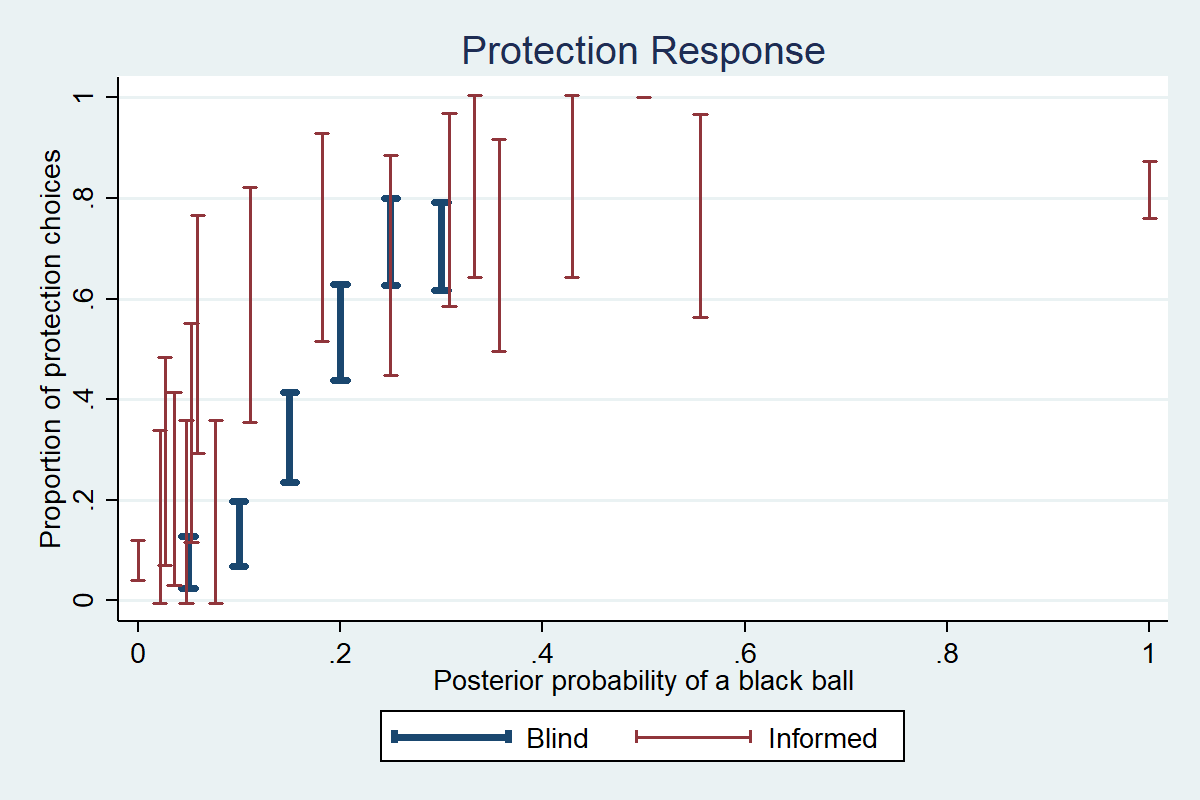
\includegraphics[width=\textwidth]{Graphs/ip_response_comp.png}
\end{subfigure}
%\begin{subfigure}[t]{.48\textwidth}
  %\centering
  %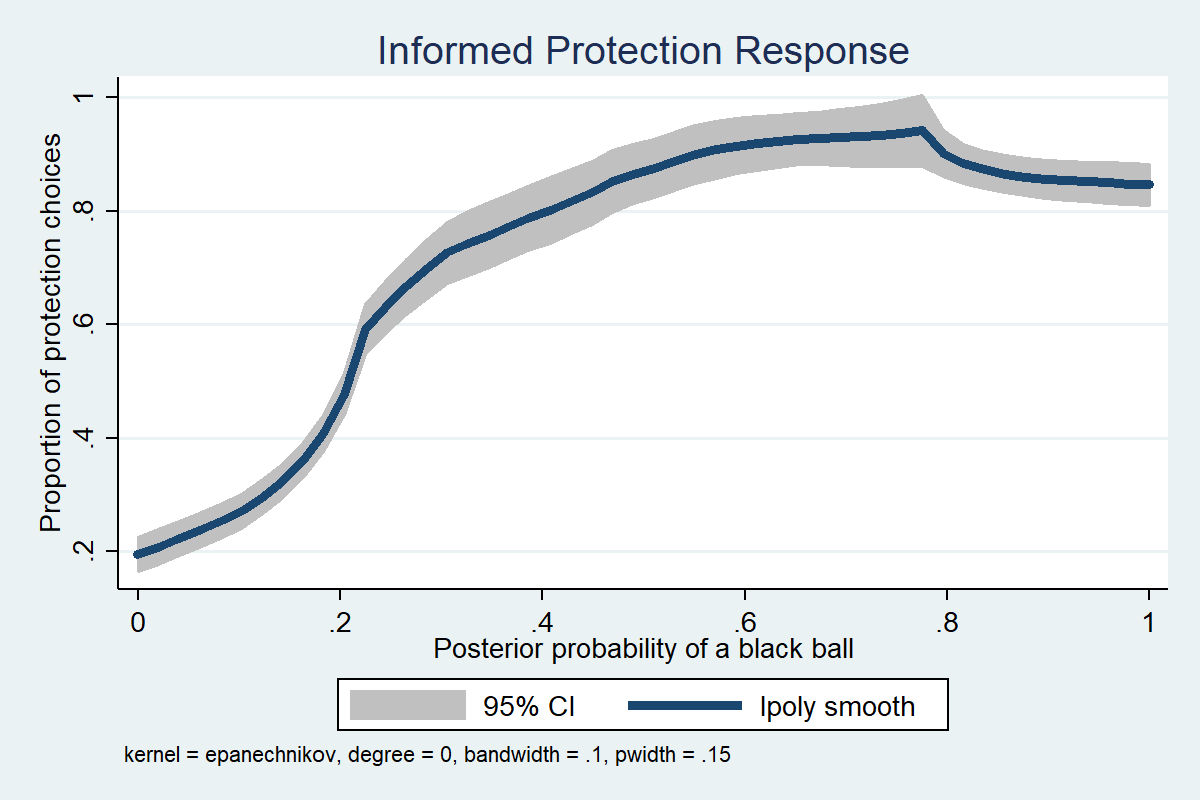
\includegraphics[width=\textwidth]{Graphs/ip_response_lpoly.png}
%
%\end{subfigure}
\end{figure}

%%%%%%%%%%%%%%%%%%%%%%%%%%%%%%%%%%%%%%%%%%%%%%%%%%%%%%%%%%%%%%%%%%%%%%%%%%%%%%%%%%%%%%%%%%%%%%%%%%%%%%%%%%%%%%%%%%%

\bigskip\noindent\textbf{Bayesian Updating Accuracy.}\ \ \ Since subjects were only given signal characteristics and not true posteriors, their IP responses reflect, inter alia, their ability to infer the true posteriors from signal characteristics. 
Figure~\ref{fig:BeliefUpdate} presents subjects' abilities to update their beliefs based on the BE task. We define updating errors as the difference between the posterior and subjects’ elicited belief on the posterior probability of a black ball for a given signal. Figure~\ref{fig:BeliefUpdate}a presents the distribution of these differences. The distribution of updating errors is centered at 0. Figure ~\ref{fig:BeliefUpdate}b presents the scatter plot of the elicited belief and the true posterior probability for a given signal. The correlation between elicited belief and the true posterior was XXXX . 

We can group the treatments in the BE task into: (i) those where the posterior is uncertain (between zero and one); and (ii) those where the posterior is certain (either zero or one). In Figure~\ref{fig:BeliefUpdate}c, we plot the distribution of updating errors for the first group of treatments. Its mean is negative, suggesting that subjects tend to overestimate the likelihood of adverse events for uncertain posteriors. The correlation between their belief and the true posterior in this subset of observations is XXX.
 
Figure~\ref{fig:BeliefUpdate}e plots the distribution of updating errors with certain posteriors, which includes: (i) treatments with all-honest gremlins; and (ii) treatments with dishonest gremlins (e.g., a group with honest and white-eyed gremlins with a hint that the ball is black — or vice versa). With perfectly honest signals, responses were incorrect for about 20 percent of the time. About half of these involve reporting a probability of between one and zero, with the other half reporting a probability of one when it should have been zero. For the latter case, only 51 percent of responses were correct. 

%%%%%%%%%%%%%%%%%%%%%%%%%%%%%%%%%%%%%%%%%%%%%%%%%%%%%%%%%%%%%%%%%%%%%%%%%%%%%%%%%%%%%%%%%%%%%%%%%%%%%%%%%%%%%%%%%%%

\begin{figure}[H]
	\centering
	\caption{Errors in Bayesian Updating} \label{fig:BeliefUpdate}
	\subcaptionbox{Error Distribution}{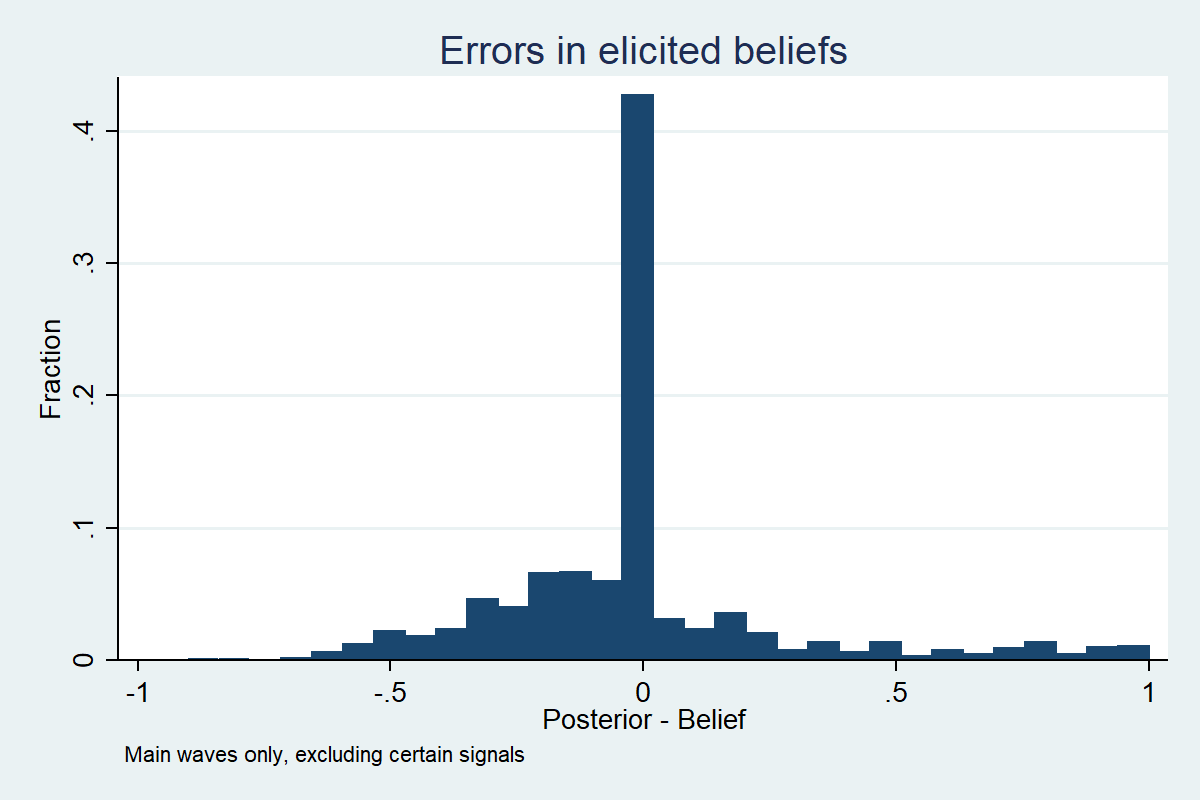
\includegraphics[width=.48\textwidth]{Graphs/hist_belief_error_s3.png}}
	\hfill
	\subcaptionbox{Error v. Posterior}{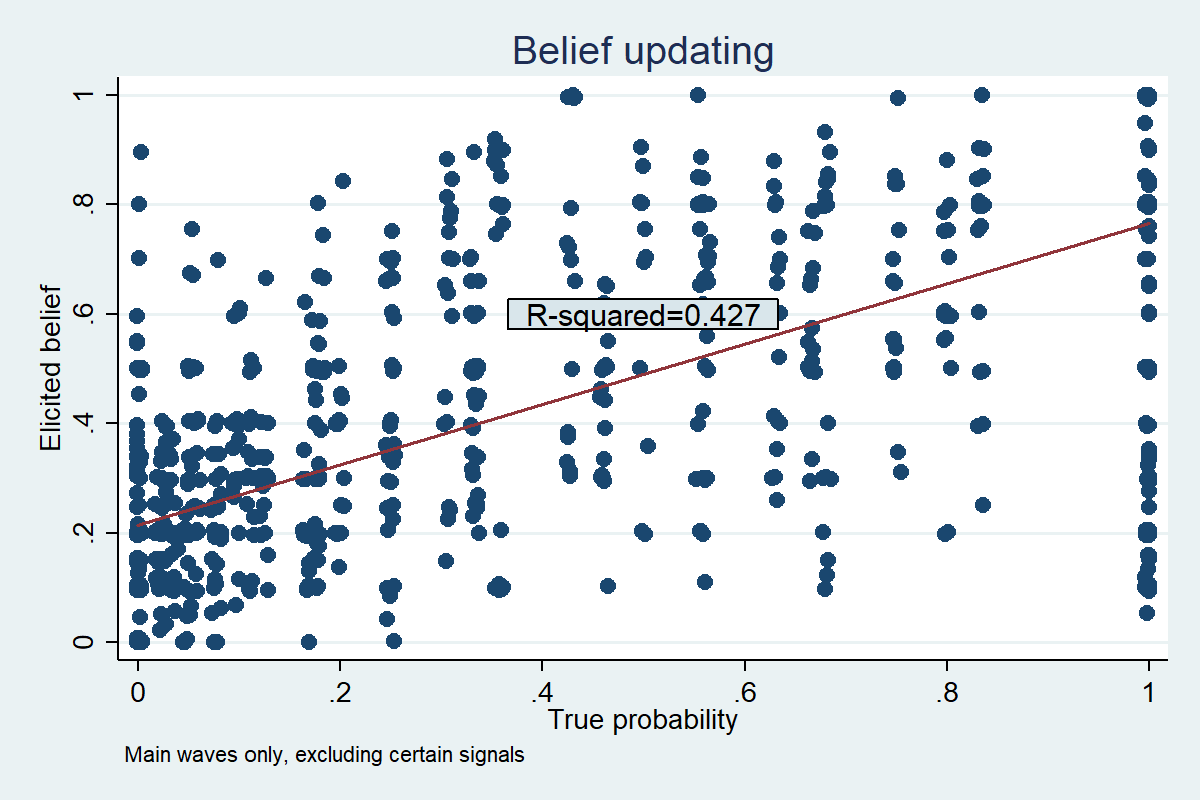
\includegraphics[width=.48\textwidth]{Graphs/updating_s3.png}}
	\hfill
	\subcaptionbox{Error Distribution, Uncertain Color}{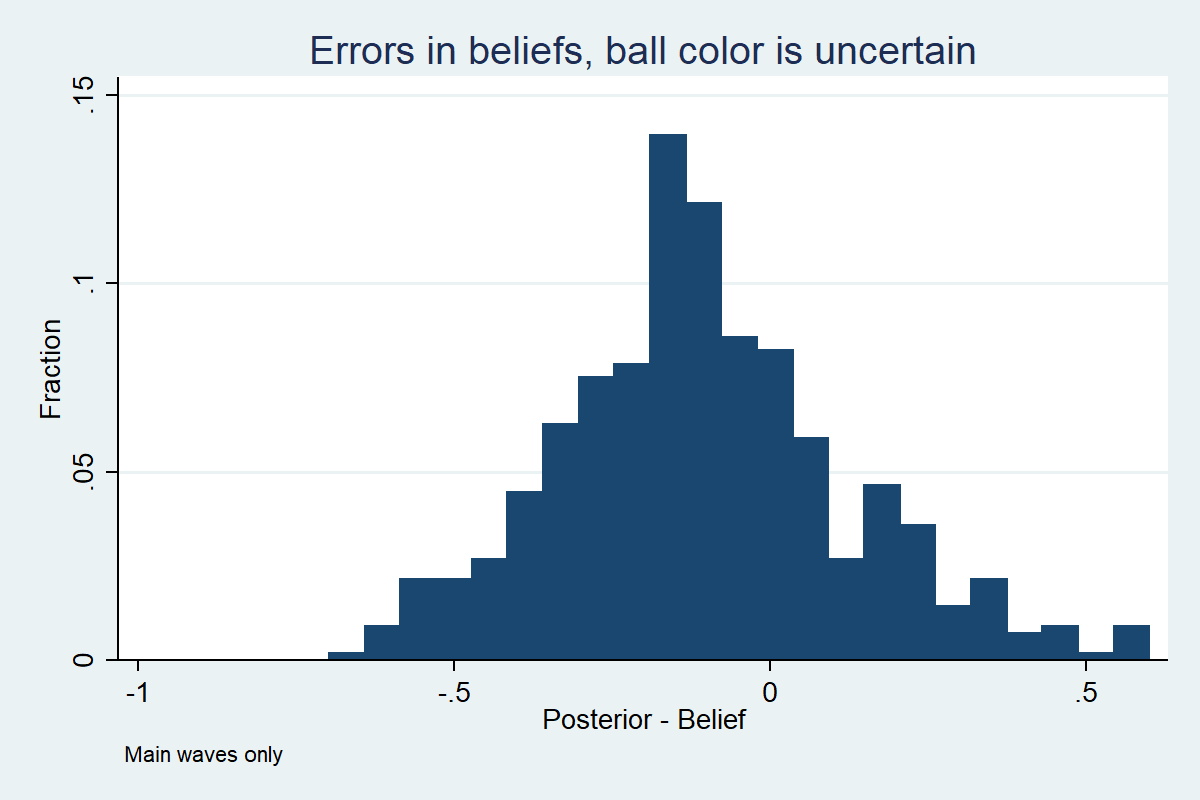
\includegraphics[width=.48\textwidth]{Graphs/hist_belief_error_s4.png}}
	\hfill
	\subcaptionbox{Error v. Posterior, Uncertain Color}{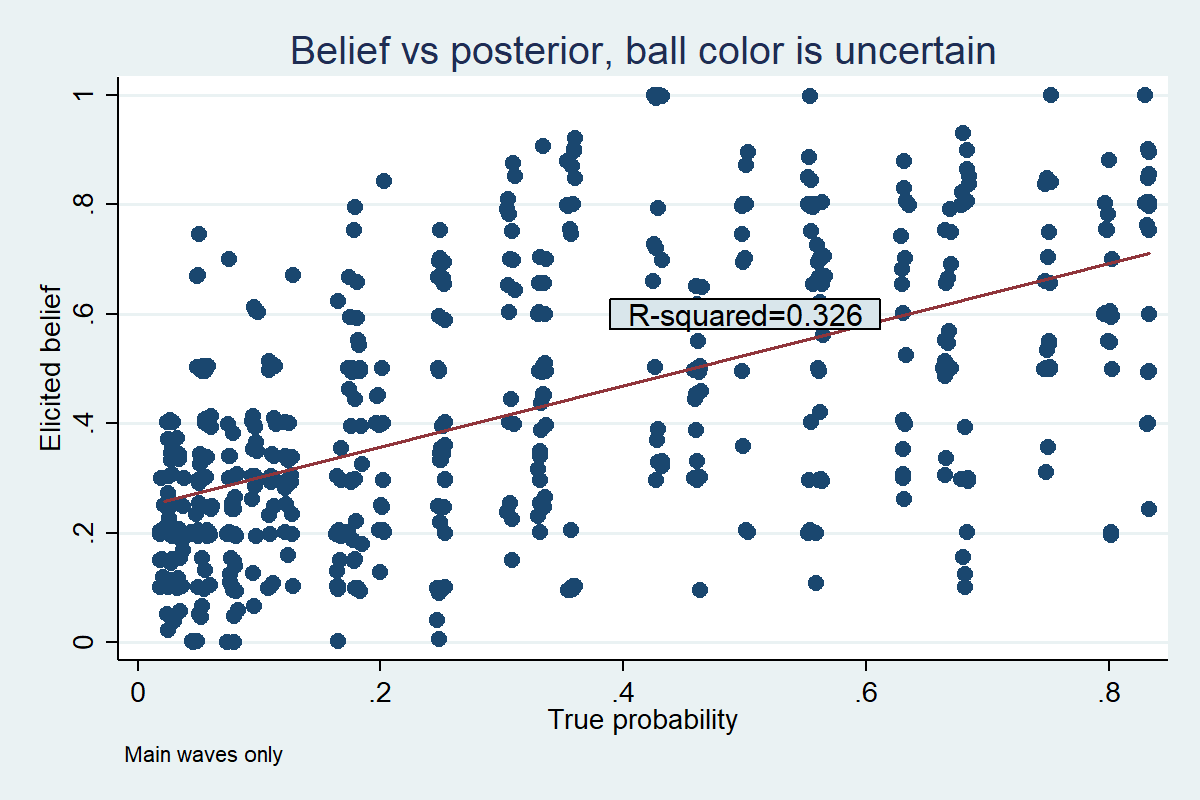
\includegraphics[width=.48\textwidth]{Graphs/updating_s4.png}}
	\hfill
	\subcaptionbox{Error Distribution, Certain Color}{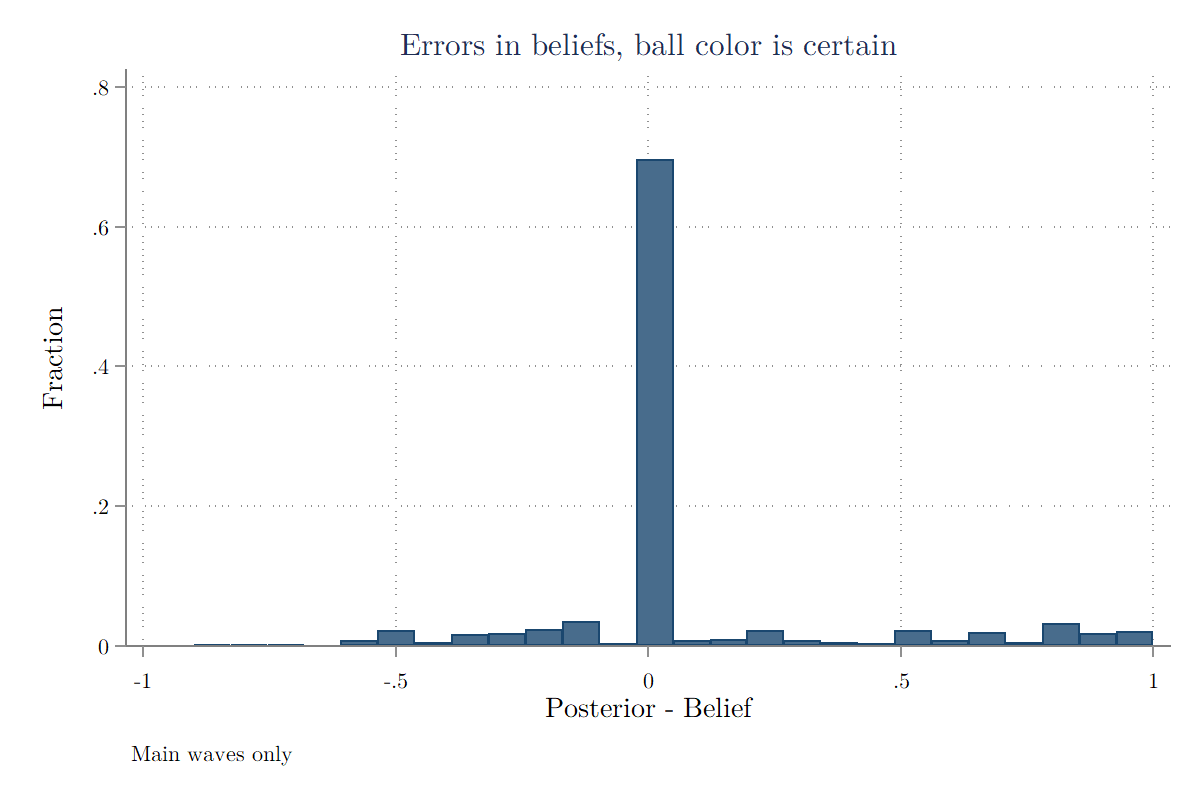
\includegraphics[width=.48\textwidth]{Graphs/hist_belief_error_s5.png}}
	\hfill
	\subcaptionbox{Error v. Posterior, Certain Color}{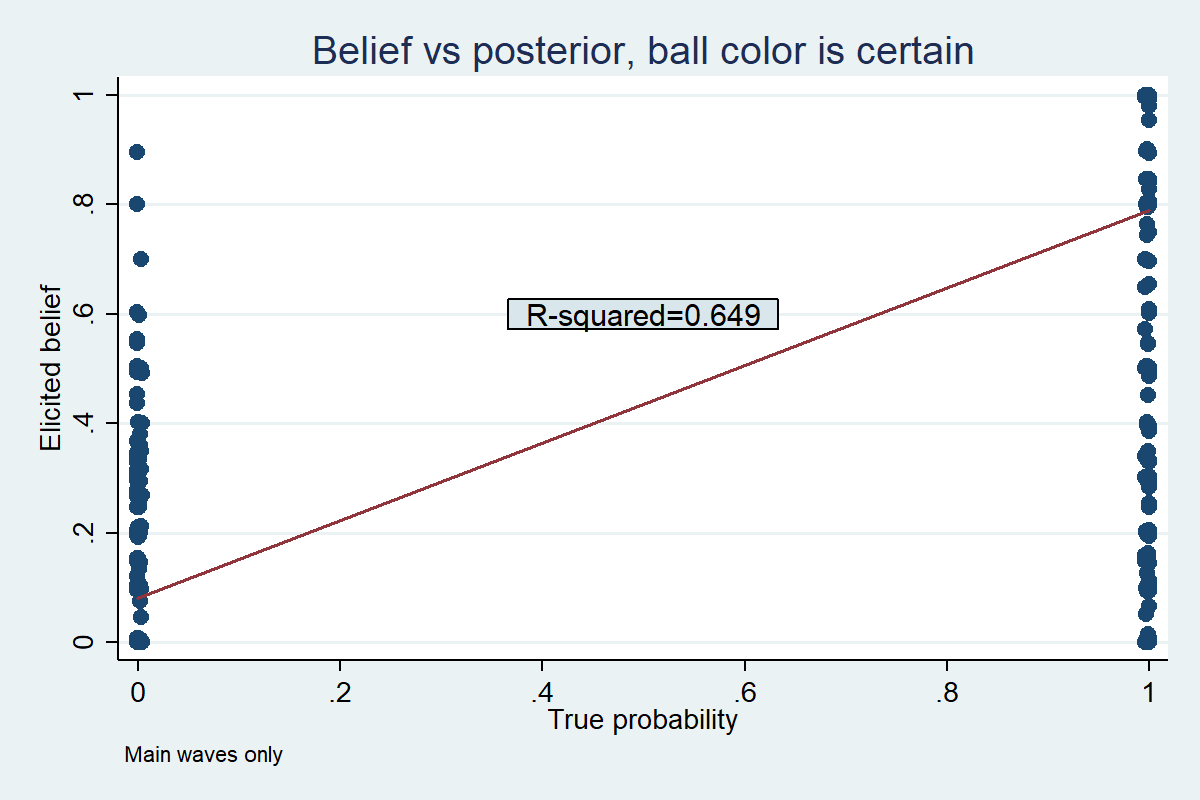
\includegraphics[width=.48\textwidth]{Graphs/updating_s5.png}}
	\hfill
\end{figure}
\clearpage

%%%%%%%%%%%%%%%%%%%%%%%%%%%%%%%%%%%%%%%%%%%%%%%%%%%%%%%%%%%%%%%%%%%%%%%%%%%%%%%%%%%%%%%%%%%%%%%%%%%%%%%%%%%%%%%%%%%



\subsection{Signal Characteristics and Protection Decision}

\textcolor{red}{XXX WE NEED TO JUSTIFY SOMEWHERE THAT WE LIMIT OUR SAMPLE TO 0.1, 0.2 FOR THE MAIN ANALYSIS STARTING FROM HERE XXX}


\begin{hypothesis} Conditional on posterior \agt{XXX and risk preferences?? XXX}, signal characteristics do not affect protection decisions. \end{hypothesis}
\begin{result}\label{res:IPdeviations} Signal characteristics affect protection decision. Conditional on posterior \agt{XXX and risk preferences?? XXX}, subjects' protection decisions still respond to the signals' false positive and false negative rates. \end{result}

Table~\ref{tab:nonparIP} presents a non-parametric analysis of subjects' IP decisions by signal characteristics (columns 1--3). Column 4 shows the \agt{XXX ALEX: How do we construct the posterior for multiple treatments? Averaging them? XXX} . Column 5 shows the share of IP responses that chose to protect, with column 6 showing the p-value of a \emph{t-}test that nobody protected. Column 7 shows... \agt{XXX ALEX: Also how do we calculate the optimal? Please add explanation XXX}, with column 8 showing the p-value of a \emph{t-}test that the share who protected is equal to the optimal share.

Overall, subjects' protection decisions deviated from what are optimal for the risk-neutral subject and these deviations systematically depend on FP and FN rates. These deviations systematically different between white and black signals. Subjects overprotected (compared to the optimal) in response to FP rates when the signal is white (rows 1--4). For example, consider the change in the protection rates between rows 1 and 3: because the signal is white, an increase in the signal's FP rate did not change the posterior. However, the protection rate increased by more than 11 percentage point (pp.). Similarly, row 4 shows that when both FP and FN are positive, the protection rate increased to 43 pp. --- even though the average (maximum) posterior probability for the signal characteristics is 6~(11) percent. As a benchmark, only 13~(32) percent of subjects chose to protect in the BP task when the probability is 10~(15) percent. 

Meanwhile, rows 5--8 show that when the signal is black, subjects protected less than what was optimal for a risk-neutral agent. However, unlike for the white signal, it appears that subjects are less responsive to changes in FP and FN rates.
%, but it doesn’t contradict EU maximization - a comparable proportion of subjects do not protect in response to honest black signals and there is no benchmark in the BP task which stops at 30% prior (for which ab 70% of subjects protect).

%%%%%%%%%%%%%%%%%%%%%%%%%%%%%%%%%%%%%%%%%%%%%%%%%%%%%%%%%%%%%%%%%%%%%%%%%%%%%%%%%%%%%%%%%%%%%

\begin{table}[H]\centering 
\caption{Average Protection by Signal Type} 
\label{tab:nonparIP}
\adjustbox{max width=\textwidth}{
	\begin{threeparttable}
	\begin{tabular}{ccccccccc} \hline \hline
	\multirow{4}{6ex}{\centering \textbf{Row}}
			&\multicolumn{3}{c}{\centering \textbf{Signal Characteristics}} 
			& \multirow{3}{10ex}{\centering \textbf{Posterior}} & \multirow{3}{10ex}{\centering \textbf{Share Protect}} 
			& \multirow{3}{13ex}{\centering \textbf{P-val $(H_0: ShProt = 0)$}} 
			& \multirow{3}{10ex}{\centering \textbf{Share Optimal}} 
			& \multirow{3}{13ex}{\centering \textbf{P-val $(H_0: ShProt=ShOptimal)$}} \\ 
			\cmidrule(lr){2-4}
		&\multirow{2}{10ex}{\centering \textbf{False Positive}} & \multirow{2}{12ex}{\centering \textbf{False Negative}} 
			& \multirow{2}{10ex}{\centering \textbf{Signal}} 
		\\
		\\
		&(1) & (2) & (3) & (4) & (5) & (6) & (7) & (8) \\
		\hline
			(1)&No&No  &White&0.000&0.067&0.000&0.000\\
(2)&No&Yes &White&0.100&0.333&0.000&0.000\\
(3)&Yes&No &White&0.000&0.130&0.000&0.000\\
(4)&Yes&Yes&White&0.131&0.564&0.121&0.000\\
(5)&No&No  &Black&1.000&0.846&1.000&0.000\\
(6)&No&Yes &Black&1.000&0.841&1.000&0.000\\
(7)&Yes&No &Black&0.550&0.833&0.870&0.355\\
(8)&Yes&Yes&Black&0.483&0.886&0.871&0.685\\

			\\
		\hline\hline 
	\end{tabular} 
	\begin{tablenotes}[flushleft]
			\item\leavevmode\kern-\scriptspace\kern-\labelsep \footnotesize \textit{Notes:} 
	\end{tablenotes}								
	\end{threeparttable}
	}
\end{table}



%%%%%%%%%%%%%%%%%%%%%%%%%%%%%%%%%%%%%%%%%%%%%%%%%%%%%%%%%%%%%%%%%%%%%%%%%%%%%%%%%%%%%%%%%%%%%


\begin{hypothesis} Subjects' Bayesian-updating errors explain IP decisions. \end{hypothesis}
\begin{result} When subjects received a signal that the ball is white, the signal's false positive and false negative rates biased their belief upward. When subjects received a signal that the ball is black, the signal's false positive (negative) rates biased their belief upward (downward). Updating errors provide partial explain for subjects' IP decisions conditional on posterior.\end{result}

Deviations from the optimal IP response can arise from subjects' failure to correctly update their posteriors. Table~\ref{tab:nonparIP} summarizes how the updating errors vary with signal characteristics. We find that when presented with a white signal, subjects failed to fully downward-adjust the likelihood of a black ball, biasing their estimates of the posterior upward. Introducing FP rates to the signal exacerbated their upward bias. To illustrate, consider the change between rows 1 and 3, where introducing an FP rate would not change the posterior (= 0) since the signal is white. Yet, subjects updated their posterior upward, magnifying their updating error. The FN rates also have a similar effect of exacerbating this upward bias for a white signal.

Meanwhile, subjects underestimated the increase in posterior when the signal is black. As in the case of the white signal, introducing FP rates led subjects to overestimate the posterior instead. In contrast, introducing FN rates led subjects to further underestimate the posterior. To illustrate, we can examine rows 5 and 6, where the introduction of an FN rate given a black signal would not change the posterior --- yet, subjects updated their posterior downward.

Table~\ref{tab:updateErrorReg} formalizes our analysis using a regression. We estimated \agt{XXX ALEX: presumably these are linear but just to be sure, can you fill this in. Thanks! XXXX}. It confirms our findings that: (i) subjects made positive (negative) updating errors for white (black) signals; (ii) FP rates induced an upward bias in subjects' estimates of the posterior; and (iii) FN rates induced an upward (downward) bias when the signal is white (black). 

%%%%%%%%%%%%%%%%%%%%%%%%%%%%%%%%%%%%%%%%%%%%%%%%%%%%%%%%%%%%%%%%%%%%%%%%%%%%%%%%%%%%%%%%%%%%%

\begin{table}[H]\centering 
\caption{Average Updating Error by Signal Type} 
\label{tab:nonparError}
\adjustbox{max width=\textwidth}{
	\begin{threeparttable}
	\begin{tabular}{ccccccc} 
	\hline \hline
 \multirow{4}{6ex}{\centering \textbf{Row}}& \multicolumn{3}{c}{\centering \textbf{Signal Characteristics}}
			& \multirow{3}{10ex}{\centering \textbf{Posterior}}  
			& \multirow{3}{12ex}{\centering \textbf{Updating Error$^*$}} & \multirow{3}{12ex}{\centering \textbf{P-val $(H_0: Error = 0)$}}  \\ \cmidrule(lr){2-4}
		& \multirow{2}{10ex}{\centering \textbf{False Positive}} & \multirow{2}{12ex}{\centering \textbf{False Negative}} 
			& \multirow{2}{10ex}{\centering \textbf{Signal}} 
		\\
		\\
		& (1) & (2) & (3) & (4) & (5) \\
	
		\hline	
1&No&No&White&0.000&0.039&0.001\\
2&No&Yes&White&0.045&0.140&0.000\\
3&Yes&No&White&0.000&0.116&0.000\\
4&Yes&Yes&White&0.062&0.245&0.000\\
5&No&No&Black&1.000&-0.187&0.000\\
6&No&Yes&Black&1.000&-0.332&0.000\\
7&Yes&No&Black&0.396&0.177&0.000\\
8&Yes&Yes&Black&0.328&0.192&0.000\\
\\ 	[-1em]
\hline\hline
\end{tabular} 
	\begin{tablenotes}[flushleft]
			\item\leavevmode\kern-\scriptspace\kern-\labelsep \footnotesize \textit{Notes:} $^* \text{Updating error} = Posterior - Belief$. 
	\end{tablenotes}								
	\end{threeparttable}
	}
\end{table}
%%%%%%%%%%%%%%%%%%%%%%%%%%%%%%%%%%%%%%%%%%%%%%%%%%%%%%%%%%%%%%%%%%%%%%%%%%%%%%%%%%%%%%%%%%%%%



%%%%%%%%%%%%%%%%%%%%%%%%%%%%%%%%%%%%%%%%%%%%%%%%%%%%%%%%%%%%%%%%%%%%%%%%%%%%%%%%%%%%%%%%%%%%%

\begin{table}[htbp]\centering 
\caption{Updating Errors in BE Task} 
\label{tab:updateErrorReg}
\adjustbox{max width=\textwidth}{
	\begin{threeparttable}
	\begin{tabular}{l*{3}{c}}
	\hline\hline
									&\multirow{2}{8ex}{\centering All}&\multicolumn{2}{c}{Signal Received}\\ \cmidrule{3-4}
									&&\multicolumn{1}{c}{White}&\multicolumn{1}{c}{Black}\\
									&\multicolumn{1}{c}{(1)}&\multicolumn{1}{c}{(2)}&\multicolumn{1}{c}{(3)}\\
	\hline

	FP rate         &     .948\sym{***}&     .318\sym{***}&     1.58\sym{***}\\
                &    (0.1)         &    (0.1)         &    (0.1)         \\
FN rate         &   .00702         &      .38\sym{***}&    -.366\sym{***}\\
                &    (0.1)         &    (0.1)         &    (0.1)         \\
Constant        &    -.249\sym{***}&     .139\sym{***}&    -.636\sym{***}\\
                &    (0.0)         &    (0.0)         &    (0.0)         \\
\hline
Observations    &      624         &      312         &      312         \\
Adjusted \(R^{2}\)&     0.22         &     0.37         &     0.66         \\

	\\ [-1em]
	\hline
	Subject FE      &      Yes         &      Yes         &      Yes         \\
	\hline
	\hline\hline
	\end{tabular}
	\begin{tablenotes}[flushleft]
			\item\leavevmode\kern-\scriptspace\kern-\labelsep \footnotesize \textit{Notes:} Standard errors in parentheses. \sym{*} \(p<0.10\), \sym{**} \(p<0.05\), \sym{***} \(p<0.01\). 
	\end{tablenotes}								
	\end{threeparttable}
	}
\end{table}


%%%%%%%%%%%%%%%%%%%%%%%%%%%%%%%%%%%%%%%%%%%%%%%%%%%%%%%%%%%%%%%%%%%%%%%%%%%%%%%%%%%%%%%%%%%%%




Certain aspects in the way subjects made updating errors are consistent with how they made IP decisions. In Table~\ref{tab:protectReg}, we regress the following  \agt{XXX ALEX, can you describe the model and specify? XXX}:
	\[ MODEL \]
where ..... Columns 1 and 2 included flexible controls of the true posteriors.\footnote{\agt{XXX ALEX: Describe what the flexible controls are in the footnote XXX}}. Columns 3 and 4 added further flexible controls to account for subjects' (often incorrect) estimates of the posterior, inferred from their BE responses.\footnote{\agt{XXX ALEX: Describe how the controls for beliefs are constructed, also the flexible aspect. XXX}} The model is estimated using \agt{XXX}, with standard errors clustered at the subject level. The table presents the average marginal effect coefficients.

Columns 1 and 2 confirmed Result~\ref{res:IPdeviations}, to wit, conditional on posterior \agt{and risk preferences?? subject FE??? XXX}, IP responses are affected by FP and FN rates. For a white signal, FP and FN rates increased the tendency to overprotect; while for a black signal, only the FP rate had a similar effect \agt{XXX ALL: I am just eyeballing here, would need to formally test and just discuss the result of the test in the footnote XXX}. Column 3 suggests, however, that once we control for both the posterior and subjects' updated belief, only the effect of the FP rate for white signals persist. These results provide evidence that subjects' failure to protect optimally is largely --- albeit not entirely --- driven by their failure to correctly update their posterior given a signal.

\agt{XXX DO WE NEED COLUMNS 2 and 4? XXX}


%%%%%%%%%%%%%%%%%%%%%%%%%%%%%%%%%%%%%%%%%%%%%%%%%%%%%%%%%%%%%%%%%%%%%%%%%%%%%%%%%%%%%%%%%%%%%
\begin{table}[htbp]\centering 
\caption{Informed Protection Response} 
\label{tab:protectReg}
\adjustbox{max width=\textwidth}{
	\begin{threeparttable}	
	\begin{tabular}{l*{4}{c}}
	\hline\hline
									&\multicolumn{1}{c}{(1)}&\multicolumn{1}{c}{(2)}&\multicolumn{1}{c}{(3)}&\multicolumn{1}{c}{(4)}\\
	\hline
		
		FP rate x (S=White)&     .676\sym{***}&     .552\sym{**} &     .379\sym{*}  &     .309         \\
                &    (3.5)         &    (2.2)         &    (1.9)         &    (1.2)         \\
FN rate x (S=White)&     1.08\sym{**} &     1.57\sym{***}&     .583         &     1.04\sym{**} \\
                &    (2.3)         &    (3.3)         &    (1.2)         &    (2.1)         \\
S=Black         &      1.2\sym{**} &     2.13\sym{***}&     .706         &     1.56\sym{***}\\
                &    (2.1)         &    (3.8)         &    (1.3)         &    (2.7)         \\
FP rate x (S=Black)&    -.887         &    -1.57\sym{*}  &    -.507         &    -1.05         \\
                &   (-1.0)         &   (-1.9)         &   (-0.6)         &   (-1.4)         \\
FN rate x (S=Black)&   -.0383         &    -.372\sym{*}  &   -.0542         &    -.372\sym{*}  \\
                &   (-0.3)         &   (-1.9)         &   (-0.3)         &   (-1.7)         \\
p$=$0.2         &     .404\sym{***}&     .363\sym{***}&     .357\sym{***}&     .316\sym{***}\\
                &    (9.5)         &    (7.1)         &    (7.1)         &    (5.0)         \\
FP rate x (p=0.2)&                  &      .55\sym{*}  &                  &     .405         \\
                &                  &    (1.7)         &                  &    (1.2)         \\
FN rate x (p=0.2)&                  &     .518\sym{*}  &                  &      .52\sym{*}  \\
                &                  &    (1.8)         &                  &    (1.8)         \\
\hline
N               &      582         &      582         &      582         &      582         \\
Pseudo R-squared&     .575         &     .585         &     .609         &     .617         \\
Log-likelihood  &     -172         &     -168         &     -158         &     -154         \\
	
	\\ [-1em]
	\hline
	Subject FE & Yes & Yes & Yes & Yes \\
	Flexible controls for: \\
	\hspace{1.5ex} Posterior & Yes & Yes & Yes & Yes \\
	\hspace{1.5ex} Beliefs & No & No & Yes & Yes \\	
	\hline\hline
	\end{tabular}
	\begin{tablenotes}[flushleft]
			\item\leavevmode\kern-\scriptspace\kern-\labelsep \footnotesize \textit{Notes:} Coefficients are average marginal effects. \emph{t}-statistics in parentheses. Standard errors are clustered at the subject level. \sym{*} \(p<0.10\), \sym{**} \(p<0.05\), \sym{***} \(p<0.01\). \agt{XXX ALEX: WHY ARE THERE 1224 OBSERVATIONS IN COLUMN 1. ARE THESE ALL OBSERVATIONS, WHILE 2-4 ARE ONLY P=0.1/0.2? XXX} 
	\end{tablenotes}								
	\end{threeparttable}
	}
\end{table}



%%%%%%%%%%%%%%%%%%%%%%%%%%%%%%%%%%%%%%%%%%%%%%%%%%%%%%%%%%%%%%%%%%%%%%%%%%%%%%%%%%%%%%%%%%%%%


\newpage\clearpage

\agt{XXX ARYA STOPPED HERE XXX}

\subsection{Willingness to Pay}

Figure XX shows how subjects deviate substantially from the theoretical value for a risk-neutral subject. Here we explore these deviations more systematically by signal characteristics and risk preferences. 

%%%%%%%%%%%%%%%%%%%%%%%%%%%%%%%%%%%%%%%%%%%%%%%%%%%%%%%%%%%%%%%%%%%%%%%%%%%%%%%%%%%%%%%%%%%%%%%%%

\begin{table}[htbp]\centering
\def\sym#1{\ifmmode^{#1}\else\(^{#1}\)\fi}
\caption{WTP for Information (tobit)}
\begin{tabular}{l*{6}{c}}
\hline\hline
                &\multicolumn{1}{c}{(1)}&\multicolumn{1}{c}{(2)}&\multicolumn{1}{c}{(3)}&\multicolumn{1}{c}{(4)}&\multicolumn{1}{c}{(5)}&\multicolumn{1}{c}{(6)}\\
                &\multicolumn{1}{c}{All}&\multicolumn{1}{c}{p=0.1}&\multicolumn{1}{c}{p=0.2}&\multicolumn{1}{c}{All}&\multicolumn{1}{c}{All}&\multicolumn{1}{c}{All}\\
\hline
model           &                  &                  &                  &                  &                  &                  \\
FN costs        &    -.577\sym{**} &    -1.24\sym{**} &    -.682\sym{***}&    -.791\sym{***}&    -.691\sym{***}&     -.69\sym{***}\\
                &    (0.2)         &    (0.5)         &    (0.3)         &    (0.2)         &    (0.2)         &    (0.3)         \\
FP costs        &    -.644\sym{***}&    -.647\sym{***}&    -.519\sym{**} &    -.595\sym{***}&    -.508\sym{***}&    -.494\sym{**} \\
                &    (0.2)         &    (0.2)         &    (0.3)         &    (0.2)         &    (0.2)         &    (0.2)         \\
BP costs        &                  &                  &                  &     .373\sym{***}&     .363\sym{***}&      .37\sym{***}\\
                &                  &                  &                  &    (0.1)         &    (0.1)         &    (0.1)         \\
Belief change   &                  &                  &                  &                  &     .332         &                  \\
                &                  &                  &                  &                  &    (0.3)         &                  \\
Certainty       &                  &                  &                  &                  &                  &     .688         \\
                &                  &                  &                  &                  &                  &    (0.8)         \\
Constant        &     1.98\sym{***}&     1.79\sym{***}&     2.33\sym{***}&     .923\sym{***}&     .701\sym{*}  &     .293         \\
                &    (0.2)         &    (0.2)         &    (0.2)         &    (0.3)         &    (0.4)         &    (0.8)         \\
\hline
sigma           &                  &                  &                  &                  &                  &                  \\
Constant        &      1.8\sym{***}&     1.83\sym{***}&      1.7\sym{***}&     1.77\sym{***}&     1.76\sym{***}&     1.76\sym{***}\\
                &    (0.1)         &    (0.1)         &    (0.1)         &    (0.1)         &    (0.1)         &    (0.1)         \\
\hline
Observations    &      312         &      159         &      153         &      312         &      312         &      312         \\
Adjusted \(R^{2}\)&                  &                  &                  &                  &                  &                  \\
\hline\hline
\multicolumn{7}{l}{\footnotesize Standard errors in parentheses}\\
\multicolumn{7}{l}{\footnotesize \sym{*} \(p<0.10\), \sym{**} \(p<0.05\), \sym{***} \(p<0.01\)}\\
\end{tabular}
\end{table}


%%%%%%%%%%%%%%%%%%%%%%%%%%%%%%%%%%%%%%%%%%%%%%%%%%%%%%%%%%%%%%%%%%%%%%%%%%%%%%%%%%%%%%%%%%%%%%%%%


In Table XX, we use a regression analysis to investigate how and why subjects deviate from the risk-neutral subjects’ theoretical WTP for a signal of a given quality (conditional on prior). We first estimate how individual deviations from the theoretical benchmark $b^*_s$ for a given signal $s$ are correlated with signal's charactaristics:

\[b_{is} - b^*_s = \beta_0 + \beta_1 FalsePositive + \beta_2 FalseNegative + \epsilon_{is}\]
where $b_{is}$ is the reported WTP of individual $i$ for treatment $s$ and $b^*_s$ is the signal's value for a risk-neutral subject, and FalsePositive (FalseNegative) is the false positive (false positive) costs variables that captures signal quality. We calculate false positive costs as the product of prior probability of a white ball multiplied by the conditional probability of getting a black signal (“The ball is black!”) from a randomly chosen gremlin: $FalsePositive=(1-\pi) P_{10}c$. Similarly we calculate false negative costs as the probability of an adverse state multiplied by a conditional probability of getting a white signal conditional on the ball being black and multiplied by potential loss $FalseNegative=\pi P_{01}L$. Note that these costs already account for expected frequency of receiving different incorrect signals as consistent with their base rate. If our subjects were risk neutral expected utility maximizers, we expect $\beta_1$ and $\beta_2$ to be zero.

%%%%%%%%%%%%%%%%%%%%%%%%%%%%%%%%%%%%%%%%%%%%%%%%%%%%%%%%%%%%%%%%%%%%%%%%%%%%%%%%%%%%%%%%%%%%%%%%%
\begin{table}[H]\centering \caption{Average WTP discrepancy (WTP-Value) by Signal Type} 
\label{tab:WTP_nonpar}
\begin{tabular}{cccc} \hline \hline
\textbf{False-positive}&\textbf{False-negative}&\textbf{Mean WTP discrepancy}& \textbf{P($=0$)}\\ \hline
No&No&-0.106&0.433\\
No&Yes&0.143&0.250\\
Yes&No&0.081&0.502\\
Yes&Yes&0.492&0.000\\
\hline \end{tabular} \end{table}

\begin{table}[H]\centering
\def\sym#1{\ifmmode^{#1}\else\(^{#1}\)\fi}
\caption{WTP minus Value of Information (OLS)}
\begin{tabular}{l*{5}{c}}
\hline\hline
                &\multicolumn{1}{c}{(1)}&\multicolumn{1}{c}{(2)}&\multicolumn{1}{c}{(3)}&\multicolumn{1}{c}{(4)}&\multicolumn{1}{c}{(5)}\\
                &\multicolumn{1}{c}{}&\multicolumn{1}{c}{}&\multicolumn{1}{c}{}&\multicolumn{1}{c}{}&\multicolumn{1}{c}{}\\
\hline
FP costs        &     .564\sym{***}&     .473\sym{***}&     .403         &     .502\sym{***}&     .435\sym{***}\\
                &    (0.1)         &    (0.1)         &    (0.3)         &    (0.2)         &    (0.1)         \\
FN costs        &     -.22\sym{*}  &    .0351         &    -.495         &    .0816         &     -.62\sym{***}\\
                &    (0.1)         &    (0.1)         &    (0.5)         &    (0.1)         &    (0.2)         \\
Risk-loving     &                  &                  &        0         &                  &                  \\
                &                  &                  &      (.)         &                  &                  \\
Risk-averse     &                  &                  &        0         &                  &                  \\
                &                  &                  &      (.)         &                  &                  \\
No risk av. measure&                  &                  &        0         &                  &                  \\
                &                  &                  &      (.)         &                  &                  \\
Risk-loving $\times$ FP costs&                  &                  &      .12         &                  &                  \\
                &                  &                  &    (0.4)         &                  &                  \\
Risk-averse $\times$ FP costs&                  &                  &     .104         &                  &                  \\
                &                  &                  &    (0.3)         &                  &                  \\
No risk av. measure $\times$ FP costs&                  &                  &    -.142         &                  &                  \\
                &                  &                  &    (0.4)         &                  &                  \\
Risk-loving $\times$ FN costs&                  &                  &     .744         &                  &                  \\
                &                  &                  &    (0.5)         &                  &                  \\
Risk-averse $\times$ FN costs&                  &                  &     .552         &                  &                  \\
                &                  &                  &    (0.5)         &                  &                  \\
No risk av. measure $\times$ FN costs&                  &                  &     .492         &                  &                  \\
                &                  &                  &    (0.5)         &                  &                  \\
Inaccurate beliefs&                  &                  &                  &    .0678         &                  \\
                &                  &                  &                  &    (0.2)         &                  \\
Inaccurate beliefs $\times$ FP costs&                  &                  &                  &     .636         &                  \\
                &                  &                  &                  &    (0.8)         &                  \\
Inaccurate beliefs $\times$ FN costs&                  &                  &                  &   .00218         &                  \\
                &                  &                  &                  &    (0.3)         &                  \\
plevel=200      &                  &                  &                  &                  &        0         \\
                &                  &                  &                  &                  &      (.)         \\
plevel=200 $\times$ FP costs&                  &                  &                  &                  &     .141         \\
                &                  &                  &                  &                  &    (0.2)         \\
plevel=200 $\times$ FN costs&                  &                  &                  &                  &     .816\sym{***}\\
                &                  &                  &                  &                  &    (0.2)         \\
Constant        &    -.108         &    -.152\sym{*}  &    -.149\sym{*}  &    -.211         &    -.123         \\
                &    (0.2)         &    (0.1)         &    (0.1)         &    (0.2)         &    (0.1)         \\
\hline
Observations    &      315         &      315         &      315         &      315         &      315         \\
Adjusted \(R^{2}\)&     0.05         &     0.59         &     0.59         &     0.59         &     0.60         \\
\hline\hline
\multicolumn{6}{l}{\footnotesize Standard errors in parentheses}\\
\multicolumn{6}{l}{\footnotesize \sym{*} \(p<0.10\), \sym{**} \(p<0.05\), \sym{***} \(p<0.01\)}\\
\end{tabular}
\end{table}

%%%%%%%%%%%%%%%%%%%%%%%%%%%%%%%%%%%%%%%%%%%%%%%%%%%%%%%%%%%%%%%%%%%%%%%%%%%%%%%%%%%%%%%%%%%%%%%%%



Column 1 of Table XX confirms that subjects’ WTP deviated from the theoretical benchmark. Subjects did not fully account for signal quality, resulting in overpaying for signals with either high false-positive and false-negative costs. Naturally, two potential sources of deviations from this theoretical benchmark based on a risk-neutral Bayesian updater are subjects’ risk-preferences and their ability to perform Bayesian updating. To test for these mechanisms, we interacted the false positive (FP) and false negative (FN) variables with individual risk aversion, whether individuals have accurate belief (as measured by our BE task), and the different priors.

Column 2 shows the results of the regression where the signal quality variables were interacted with the subject’s risk preference.\footnote{Our risk preference estimates come from blind protection choice: subjects switching from no protection to protection at exactly the cost-loss ratio $\pi=0.2$ are considered risk-neutral, while switching at lower (higher) levels indicates risk aversion (risk-loving).} This premium doesn’t seem to come from risk aversion, as the coefficient on the interaction of risk aversion with FP and FN rates is relatively small and insignificant. Belief accuracy measured in the belief elicitation task apparently explains away the excess sensitivity to the FP rate but this finding should be taken with caution because the coefficient is not statistically significant despite its large absolute magnitude.

These results suggest that, on average, subjects failed to fully account for signal quality, resulting in overpaying for signals with high false-positive and false-negative costs.  FP/FN significantly impact the deviation from the theoretical value no matter what else is included.  

%Another plausible explanation would be that subjects are engaging in some sort of probability weighting depending on the priors along the line of XXXX.  In Column 5, we find that …. Probability weighting involves making decisions not based on actual probabilities but on transformed probabilities. Typical transformation is mapping low probability to higher probabilities and very high probabilities to lower, resulting in compressing the distribution more towards 0.5. For example, a subject can react to an event with 0.05 probability as if it is an event with 0.15 probability.  Finally, we consider the signal characteristics, i.e., do subjects deviate from the theoretical value of a signal because they imbue false positives or negatives with undue importance.
%
%Digging into these determinants of the discrepancy, Table 2 looks at the effect of FP/FN by each possible prior.  When separated this way a distinct pattern emerges: when priors are low, subjects underreact to FP rates and overreact to FN rates compared to a risk-neutral decision-maker. When priors are high, subjects do the opposite by overreacting to FN rates and underreacting to FP rates.
%
%One potential explanation for the observed pattern is that subjects do not correctly estimate the frequency of false-positive and false-negative outcomes. These frequencies are sufficient statistics for determining the signal’s value in any expected utility framework (see x). Subjects are given only false-positive rates and priors, but what matters for the signal’s value in most common frameworks including the expected utility framework, is the frequency of observing false-positive and false-negative signals. We call this bias a probability estimation bias. This bias is similar to other biases in calculating posterior probabilities such as base-rate neglect or signal neglect, but instead of failing to calculate a posterior probabilities here subjects fail to estimate the probability of a compound event given priors and conditional probabilities.

%\vspace{20pt}
%\section{Explaining Underutilization of Signal Quality}
%
%We also need to make sure that any more accepted theories of decision-making under uncertainty do not explain this pattern.  We analyze three alternative theories, including risk aversion, loss aversion and probability weighting. Both risk aversion with prudence and loss aversion can produce choices consistent with the observed pattern. Probability weighting in theory produces the pattern opposite to the observed one.
%
%WTP regressions show that subjects overpay for signals with high FP and FN rates, but is this consistent with the way they use signals?  In Table 3, we look at what influences a subject’s choice to protect in the IP treatment where they have been given a signal. For any rational subject (following one of the theories above), posterior probability provides all the information needed for making protection decisions. But we observe that even controlling for the posterior probability (with splines of the posterior prob), subjects tend to protect more when faced with signals with high false-positive or false-negative rates.\footnote{To account for the non-linearity of potential response to posterior probability, we split the domain of this variable in 5 equal segments. Then we add 5 linear splines, so that each variable is equal to the posterior probability when the posterior probability is inside the corresponding segment and zero otherwise.} 
%
%WTP regressions show that subjects overpay for signals with high FP and FN rates. Informed protection responses also demonstrate that subjects overuse bad signals. Controlling for the posterior probability (with splines of the posterior probability), subjects tend to protect more when faced with signals with high false-positive or false-negative rates.
%
%Their behavior is consistent with underweighting prior and/or signals when calculating the posterior probability. Even controlling for the posterior, subjects protect more when the prior probability is high (>0.2) (columns 3-4). For high priors, they also react less to false-positive rates but more to false-negative rates. Practically all the extra-protection in response to false-negative rates comes from white signals (as expected), but the effect of false positive rates exists both for white and black signals. 
%
%Subjects obviously do not behave as risk-neutral decision-makers when paying for signals. Which theory explains their behavior the best? We study this problem in context of different decision theories and find that several of them are consistent with the pattern (of underreacting to FP rates and overreacting to FN rates for low priors and vice versa) for certain ranges and parametrizations. Strictly risk-averse and prudent decision-makers become relatively more sensitive to false-negative rates with increasing priors as compared to risk-neutral subjects. For loss-averse subjects, the sensitivity to false-positive rates should decrease with priors due to shifting baselines. Finally, the probability estimation bias means that subjects do not correctly map reported false-positive and false-negative rates and priors into probabilities of false-positive and false-negative outcomes.
%
%Here we specifically test for the probability estimation bias versus other theories. Probability estimation bias predicts that subjects consistently react to other factors such as FP and FN rates conditional on priors and probabilities of FP and FN outcomes. Indeed we observe that even with flexible controls for priors and total probabilities, subjects reduce their WTP with increasing FP and FN rates.  
%


\subsection{Summary}

%%%%%%%%%%%%%%%%%%%%%%%%%%%%%%%%%%%%%%%%%%%%%%%%%%%%%%%%%%%%%%%%%%%%%%%%%%%%%%%%%%%%%%%%%%%%%%%%%
\begin{table}[H]\centering
\caption{Comparing Findings across the Tasks}
\begin{tabular}{l|c|c|c}
\hline \hline
Design & Beliefs & IP &WTP\\
\hline
White, FN only & $>$ & $<>$ & $<>*$ \\
Black, FN only & $<$ & $<>$ & $<>$ \\
White, FP only & $>$ & $>$ & $>$ \\
Black, FP only & $>$ & $<>$ & $>$ \\
White, FN and FP & $>>$ & $>$ & $>$ \\
Black, FN and FP & $>$ & $<>$ & $>$\\
\hline
\multicolumn{4}{l}{*-WTP estimates do not depend on signals.}\\
\end{tabular}
\end{table}


%%%%%%%%%%%%%%%%%%%%%%%%%%%%%%%%%%%%%%%%%%%%%%%%%%%%%%%%%%%%%%%%%%%%%%%%%%%%%%%%%%%%%%%%%%%%%%%%%


\newpage
\singlespacing
\small

\subsection{Subject Heterogeneity}


\begin{table}[H]
\caption{Latent Class Multinomial Choice Model Estimates (FP and FN rates by hint)}
\begin{tabular}{l*{10}{c}}
\hline\hline
            &  lc\_results&            &            &            &            &            &            &            &            &            \\
            &       Model&       Class&         Alt&        Hint&         FN0&         FN1&         FP0&         FP1& Class share&         BIC\\
\hline
r1          &           1&           1&    -2.86694&    4.392251&    4.834518&   -.1919326&     4.35168&   -.8676941&           1&    597.4337\\
r2          &           2&           1&    -2.91958&    1.881626&    7.980388&   -.3599557&    1.725487&    6.632253&    .2198715&    587.6042\\
r3          &           2&           2&    -2.91958&    6.699559&    3.838407&    .4707898&    5.285504&   -8.229022&    .7801285&    587.6042\\
\hline\hline
\end{tabular}

\end{table}

%\begin{table}[htbp]\centering
\def\sym#1{\ifmmode^{#1}\else\(^{#1}\)\fi}
\caption{IP response by class}
\begin{tabular}{l*{3}{c}}
\hline\hline
                &\multicolumn{1}{c}{(1)}&\multicolumn{1}{c}{(2)}&\multicolumn{1}{c}{(3)}\\
                &\multicolumn{1}{c}{All}&\multicolumn{1}{c}{Class 1}&\multicolumn{1}{c}{Class 2}\\
\hline
S=Black         &     .587\sym{***}&     .406\sym{***}&     .962\sym{***}\\
                &   (26.3)         &    (5.3)         &    (6.5)         \\
FN rate*White hint&     .948\sym{***}&     1.41\sym{***}&     .619\sym{***}\\
                &    (9.3)         &    (6.7)         &    (9.3)         \\
FP rate*White hint&     .435\sym{***}&     .763\sym{***}&     .277\sym{***}\\
                &    (4.0)         &    (2.8)         &    (3.4)         \\
FN rate*Black hint&   .00432         &     .327         &   -.0959         \\
                &    (0.0)         &    (1.5)         &   (-0.8)         \\
FP rate*Black hint&    .0293         &     1.03\sym{***}&    -1.68\sym{***}\\
                &    (0.2)         &    (4.2)         &   (-3.5)         \\
\hline
N               &     1248         &      336         &      912         \\
Pseudo R-squared&     .359         &     .214         &     .556         \\
Log-likelihood  &     -551         &     -179         &     -272         \\
\hline\hline
\multicolumn{4}{l}{\footnotesize \textit{t} statistics in parentheses}\\
\multicolumn{4}{l}{\footnotesize Errors are clustered by subject, average marginal treatment effects}\\
\multicolumn{4}{l}{\footnotesize \sym{*} \(p<0.10\), \sym{**} \(p<0.05\), \sym{***} \(p<0.01\)}\\
\end{tabular}
\end{table}

\begin{table}[htbp]\centering
\def\sym#1{\ifmmode^{#1}\else\(^{#1}\)\fi}
\caption{IP response by class}
\begin{tabular}{l*{2}{c}}
\hline\hline
                &\multicolumn{1}{c}{(1)}&\multicolumn{1}{c}{(2)}\\
                &\multicolumn{1}{c}{Honesty Seekers}&\multicolumn{1}{c}{Cautious Bayesians}\\
\hline
S=Black         &     .337\sym{***}&    .0245         \\
                &    (3.4)         &    (0.4)         \\
Prop. of lying gremlins&     .664\sym{***}&     .277\sym{***}\\
                &    (4.6)         &    (4.3)         \\
Posterior prob. &    -.198\sym{*}  &     .788\sym{***}\\
                &   (-1.7)         &    (4.9)         \\
\hline
N               &      138         &      486         \\
Pseudo R-squared&     .183         &     .541         \\
Log-likelihood  &    -67.2         &     -154         \\
\hline\hline
\multicolumn{3}{l}{\footnotesize \textit{t} statistics in parentheses}\\
\multicolumn{3}{l}{\footnotesize Errors are clustered by subject, average marginal treatment effects}\\
\multicolumn{3}{l}{\footnotesize \sym{*} \(p<0.10\), \sym{**} \(p<0.05\), \sym{***} \(p<0.01\)}\\
\end{tabular}
\end{table}


\begin{table}[htbp]\centering
\def\sym#1{\ifmmode^{#1}\else\(^{#1}\)\fi}
\caption{Belief Elicitation by Class}
\begin{tabular}{l*{2}{c}}
\hline\hline
                &\multicolumn{1}{c}{(1)}&\multicolumn{1}{c}{(2)}\\
                &\multicolumn{1}{c}{Simpletons}&\multicolumn{1}{c}{Cautious Bayesians}\\
\hline
Posterior prob. &     .357\sym{***}&     .479\sym{***}\\
                &    (0.1)         &    (0.1)         \\
S=Black         &     .123         &     .224\sym{***}\\
                &    (0.1)         &    (0.0)         \\
Prop. of lying gremlins&     .171         &     .184\sym{***}\\
                &    (0.1)         &    (0.0)         \\
Constant        &     .112\sym{***}&    .0898\sym{***}\\
                &    (0.0)         &    (0.0)         \\
\hline
Observations    &      138         &      486         \\
Adjusted \(R^{2}\)&     0.31         &     0.60         \\
\hline\hline
\multicolumn{3}{l}{\footnotesize Standard errors in parentheses}\\
\multicolumn{3}{l}{\footnotesize Dep. variable: beliefs, errors clustered by subject}\\
\multicolumn{3}{l}{\footnotesize \sym{*} \(p<0.10\), \sym{**} \(p<0.05\), \sym{***} \(p<0.01\)}\\
\end{tabular}
\end{table}


\begin{table}[htbp]\centering
\caption{Expected IP losses by strategy}
\begin{tabular}{l c c c|c c c}
\hline\hline
            & \multicolumn{3}{c}{p=0.1,0.2}            &     \multicolumn{3}{c}{p$>$0.2}             \\
            &   Mean loss&\% of optimal&  Loss prob.&   Mean loss&\% of optimal&  Loss prob.\\
\hline
Baseline (all)&    1.166304&    156.7689&    .0190281&     2.11717&    140.6088&    .0508233\\
Honesty seekers&    1.526998&    205.2517&    .0435806&    3.095308&    205.5705&    .1163925\\
Bayesians   &    1.050706&    141.2308&    .0112388&    1.806053&    119.9464&    .0300237\\
Optimal     &    .7439637&           1&    .0136432&    1.505716&           1&    .0190598\\
\hline\hline
\end{tabular}
\end{table}



\begin{table}[htbp]\centering
\def\sym#1{\ifmmode^{#1}\else\(^{#1}\)\fi}
\caption{Belief Elicitation: When Mistakes Happen}
\begin{tabular}{l*{3}{c}}
\hline\hline
                &\multicolumn{1}{c}{(1)}&\multicolumn{1}{c}{(2)}&\multicolumn{1}{c}{(3)}\\
                &\multicolumn{1}{c}{All}&\multicolumn{1}{c}{S=White}&\multicolumn{1}{c}{S=Black}\\
\hline
Simpletons      &    .0993\sym{***}&    -.258\sym{***}&     .457\sym{***}\\
                &    (0.0)         &    (0.0)         &    (0.0)         \\
FN rate         &    .0437         &     .279\sym{***}&    -.192\sym{**} \\
                &    (0.0)         &    (0.1)         &    (0.1)         \\
Simpletons $\times$ FN rate&     -.13         &   -.0124         &    -.248         \\
                &    (0.2)         &    (0.2)         &    (0.2)         \\
FP rate         &     .562\sym{***}&     .258\sym{***}&     .866\sym{***}\\
                &    (0.1)         &    (0.1)         &    (0.1)         \\
Simpletons $\times$ FP rate&     .171         &     .171         &      .17         \\
                &    (0.2)         &    (0.2)         &    (0.3)         \\
Constant        &   -.0802\sym{***}&     .315\sym{***}&    -.475\sym{***}\\
                &    (0.0)         &    (0.0)         &    (0.0)         \\
Subject FE      &      Yes         &      Yes         &      Yes         \\
\hline
Observations    &     1248         &      624         &      624         \\
Adjusted \(R^{2}\)&     0.15         &     0.42         &     0.52         \\
\hline\hline
\multicolumn{4}{l}{\footnotesize Standard errors in parentheses}\\
\multicolumn{4}{l}{\footnotesize Dep. variable: reported belief - posterior probability}\\
\multicolumn{4}{l}{\footnotesize \sym{*} \(p<0.10\), \sym{**} \(p<0.05\), \sym{***} \(p<0.01\)}\\
\end{tabular}
\end{table}



\section{Conclusion}


\clearpage


\bibliography{Alerts}


 
\appendix

\newpage
\section{Tables}


\begin{table}[h!]
\caption{Demographic Characteristics of Subjects} \label{summ_tab}
\begin{tabular}{l*{7}{c}}
\hline\hline
 &  \multicolumn{2}{c}{All} & \multicolumn{2}{c}{$p\in\{0.1,0.3\}$} & \multicolumn{2}{c}{$p\in\{0.2,0.5\}$} \\
\hline
 & N & \%  & N & \%  & N & \%  \\
\hline
Male         &    43 & 41  &  22  &  41 & 21  & 41  \\

Age$>$23yrs old     &    14 & 13  &  6  & 11  &8   & 16  \\

Students     &    88 & 84  &  46  & 85  &  42 &  82 \\

Had statistics classes      &    63 & 60  & 37   & 69  & 26  &  51 \\

Total     &    105 & 100  & 54   & 100   &  51 &  100 \\

\end{tabular}


\end{table}

\begin{table}[h!]
\caption{Risk Aversion Measurement} \label{ra_tab}
\begin{table}[htbp]\centering
\def\sym#1{\ifmmode^{#1}\else\(^{#1}\)\fi}
\caption{Relative risk avers distribution}
\begin{tabular}{l*{1}{c}}
\hline\hline
                    &\multicolumn{1}{c}{(1)}\\
                    &\multicolumn{1}{c}{}\\
                    &           b\\
\hline
\hline
Observations        &          25\\
Adjusted \(R^{2}\)  &            \\
\hline\hline
\end{tabular}
\end{table}

\end{table}


\begin{table}[htbp!]
\begin{table}[htbp]\centering
\def\sym#1{\ifmmode^{#1}\else\(^{#1}\)\fi}
\caption{Informed protection response: logistical regression}
\begin{tabular}{l*{6}{c}}
\hline\hline
                &\multicolumn{1}{c}{(1)}&\multicolumn{1}{c}{(2)}&\multicolumn{1}{c}{(3)}&\multicolumn{1}{c}{(4)}&\multicolumn{1}{c}{(5)}&\multicolumn{1}{c}{(6)}\\
                &\multicolumn{1}{c}{All}&\multicolumn{1}{c}{S=White}&\multicolumn{1}{c}{S=Black}&\multicolumn{1}{c}{All}&\multicolumn{1}{c}{S=White}&\multicolumn{1}{c}{W=Black}\\
\hline
FP rate         &     .248\sym{**} &     .557\sym{***}&    -.146         &     .198\sym{*}  &     1.19\sym{***}&     -.38         \\
                &    (2.2)         &    (4.8)         &   (-0.9)         &    (1.7)         &    (3.7)         &   (-0.8)         \\
FN rate         &     .341\sym{***}&      .61\sym{***}&    -.025         &      .35\sym{***}&     1.26\sym{***}&    -.116         \\
                &    (3.2)         &    (4.6)         &   (-0.2)         &    (3.2)         &   (12.8)         &   (-0.3)         \\
S=Black         &     .454\sym{***}&                  &                  &     .473\sym{***}&                  &                  \\
                &   (89.2)         &                  &                  &   (98.4)         &                  &                  \\
plevel=200      &     .105\sym{***}&     .093\sym{*}  &     .117\sym{**} &        0         &        0         &        0         \\
                &    (2.8)         &    (1.9)         &    (2.1)         &      (.)         &      (.)         &      (.)         \\
Subject FE      &       No         &       No         &       No         &      Yes         &      Yes         &      Yes         \\
\hline
P(FP rate $\neq$ FN rate)&     .524         &     .787         &     .621         &     .306         &     .855         &     .705         \\
N               &      629         &      315         &      314         &      587         &      117         &      105         \\
Pseudo R-squared&     .333         &     .161         &    .0252         &     .522         &     .479         &    .0844         \\
Log-likelihood  &     -291         &     -125         &     -152         &     -195         &    -41.2         &    -66.1         \\
\hline\hline
\multicolumn{7}{l}{\footnotesize \textit{t} statistics in parentheses}\\
\multicolumn{7}{l}{\footnotesize Errors are clustered by subject, average marginal treatment effects}\\
\multicolumn{7}{l}{\footnotesize \sym{*} \(p<0.10\), \sym{**} \(p<0.05\), \sym{***} \(p<0.01\)}\\
\end{tabular}
\end{table}

\end{table}


\begin{table}[hbp!]
\begin{table}[htbp]\centering
\def\sym#1{\ifmmode^{#1}\else\(^{#1}\)\fi}
\caption{Informed Protection Response: logit with flexible control for posteriors}
\begin{tabular}{l*{4}{c}}
\hline\hline
                &\multicolumn{1}{c}{(1)}&\multicolumn{1}{c}{(2)}&\multicolumn{1}{c}{(3)}&\multicolumn{1}{c}{(4)}\\
                &\multicolumn{1}{c}{}&\multicolumn{1}{c}{}&\multicolumn{1}{c}{}&\multicolumn{1}{c}{}\\
\hline
FP rate         &     .365\sym{***}&     .461\sym{***}&     .508\sym{**} &     .552\sym{**} \\
                &    (3.3)         &    (3.3)         &    (2.4)         &    (2.2)         \\
FN rate         &     .169\sym{*}  &     .544\sym{***}&     .181         &     1.57\sym{***}\\
                &    (1.8)         &    (2.9)         &    (1.1)         &    (3.3)         \\
p$=$0.2         &    .0637\sym{**} &     .113\sym{***}&     .313\sym{***}&     .363\sym{***}\\
                &    (2.1)         &    (4.2)         &    (7.7)         &    (7.1)         \\
S=Black         &    .0421         &      .42\sym{***}&    -.127         &     2.13\sym{***}\\
                &    (0.7)         &    (2.7)         &   (-0.9)         &    (3.8)         \\
FP rate x (S=Black)&                  &    -.716         &                  &    -2.12\sym{***}\\
                &                  &   (-1.5)         &                  &   (-3.0)         \\
FN rate x (S=Black)&                  &    -.495\sym{**} &                  &    -1.94\sym{***}\\
                &                  &   (-2.2)         &                  &   (-3.4)         \\
FP rate x (p=0.2)&                  &                  &    .0374         &      .55\sym{*}  \\
                &                  &                  &    (0.1)         &    (1.7)         \\
FN rate x (p=0.2)&                  &                  &   -.0718         &     .518\sym{*}  \\
                &                  &                  &   (-0.3)         &    (1.8)         \\
\hline
Observations    &     1248         &     1224         &      582         &      582         \\
Adjusted \(R^{2}\)&                  &                  &                  &                  \\
\hline\hline
\multicolumn{5}{l}{\footnotesize \textit{t} statistics in parentheses}\\
\multicolumn{5}{l}{\footnotesize Reporting average marginal effects, subject FE, errors are clustered by subject.}\\
\multicolumn{5}{l}{\footnotesize With flexible controls of posterior probability}\\
\multicolumn{5}{l}{\footnotesize \sym{*} \(p<0.10\), \sym{**} \(p<0.05\), \sym{***} \(p<0.01\)}\\
\end{tabular}
\end{table}
 \label{ip_tab}
\end{table}

\begin{table}[h!]
\begin{table}[htbp]\centering
\def\sym#1{\ifmmode^{#1}\else\(^{#1}\)\fi}
\caption{WTP for Information (tobit)}
\begin{tabular}{l*{6}{c}}
\hline\hline
                &\multicolumn{1}{c}{(1)}&\multicolumn{1}{c}{(2)}&\multicolumn{1}{c}{(3)}&\multicolumn{1}{c}{(4)}&\multicolumn{1}{c}{(5)}&\multicolumn{1}{c}{(6)}\\
                &\multicolumn{1}{c}{All}&\multicolumn{1}{c}{p=0.1}&\multicolumn{1}{c}{p=0.2}&\multicolumn{1}{c}{All}&\multicolumn{1}{c}{All}&\multicolumn{1}{c}{All}\\
\hline
model           &                  &                  &                  &                  &                  &                  \\
FN costs        &    -.577\sym{**} &    -1.24\sym{**} &    -.682\sym{***}&    -.791\sym{***}&    -.691\sym{***}&     -.69\sym{***}\\
                &    (0.2)         &    (0.5)         &    (0.3)         &    (0.2)         &    (0.2)         &    (0.3)         \\
FP costs        &    -.644\sym{***}&    -.647\sym{***}&    -.519\sym{**} &    -.595\sym{***}&    -.508\sym{***}&    -.494\sym{**} \\
                &    (0.2)         &    (0.2)         &    (0.3)         &    (0.2)         &    (0.2)         &    (0.2)         \\
BP costs        &                  &                  &                  &     .373\sym{***}&     .363\sym{***}&      .37\sym{***}\\
                &                  &                  &                  &    (0.1)         &    (0.1)         &    (0.1)         \\
Belief change   &                  &                  &                  &                  &     .332         &                  \\
                &                  &                  &                  &                  &    (0.3)         &                  \\
Certainty       &                  &                  &                  &                  &                  &     .688         \\
                &                  &                  &                  &                  &                  &    (0.8)         \\
Constant        &     1.98\sym{***}&     1.79\sym{***}&     2.33\sym{***}&     .923\sym{***}&     .701\sym{*}  &     .293         \\
                &    (0.2)         &    (0.2)         &    (0.2)         &    (0.3)         &    (0.4)         &    (0.8)         \\
\hline
sigma           &                  &                  &                  &                  &                  &                  \\
Constant        &      1.8\sym{***}&     1.83\sym{***}&      1.7\sym{***}&     1.77\sym{***}&     1.76\sym{***}&     1.76\sym{***}\\
                &    (0.1)         &    (0.1)         &    (0.1)         &    (0.1)         &    (0.1)         &    (0.1)         \\
\hline
Observations    &      312         &      159         &      153         &      312         &      312         &      312         \\
Adjusted \(R^{2}\)&                  &                  &                  &                  &                  &                  \\
\hline\hline
\multicolumn{7}{l}{\footnotesize Standard errors in parentheses}\\
\multicolumn{7}{l}{\footnotesize \sym{*} \(p<0.10\), \sym{**} \(p<0.05\), \sym{***} \(p<0.01\)}\\
\end{tabular}
\end{table}

\end{table}

\begin{table}[h!]
\begin{table}[htbp]\centering
\def\sym#1{\ifmmode^{#1}\else\(^{#1}\)\fi}
\caption{WTP minus Value of Information (OLS)}
\begin{tabular}{l*{5}{c}}
\hline\hline
                &\multicolumn{1}{c}{(1)}&\multicolumn{1}{c}{(2)}&\multicolumn{1}{c}{(3)}&\multicolumn{1}{c}{(4)}&\multicolumn{1}{c}{(5)}\\
                &\multicolumn{1}{c}{}&\multicolumn{1}{c}{}&\multicolumn{1}{c}{}&\multicolumn{1}{c}{}&\multicolumn{1}{c}{}\\
\hline
FP costs        &     .564\sym{***}&     .473\sym{***}&     .403         &     .502\sym{***}&     .435\sym{***}\\
                &    (0.1)         &    (0.1)         &    (0.3)         &    (0.2)         &    (0.1)         \\
FN costs        &     -.22\sym{*}  &    .0351         &    -.495         &    .0816         &     -.62\sym{***}\\
                &    (0.1)         &    (0.1)         &    (0.5)         &    (0.1)         &    (0.2)         \\
Risk-loving $\times$ FP costs&                  &                  &      .12         &                  &                  \\
                &                  &                  &    (0.4)         &                  &                  \\
Risk-averse $\times$ FP costs&                  &                  &     .104         &                  &                  \\
                &                  &                  &    (0.3)         &                  &                  \\
No risk av. measure $\times$ FP costs&                  &                  &    -.142         &                  &                  \\
                &                  &                  &    (0.4)         &                  &                  \\
Risk-loving $\times$ FN costs&                  &                  &     .744         &                  &                  \\
                &                  &                  &    (0.5)         &                  &                  \\
Risk-averse $\times$ FN costs&                  &                  &     .552         &                  &                  \\
                &                  &                  &    (0.5)         &                  &                  \\
No risk av. measure $\times$ FN costs&                  &                  &     .492         &                  &                  \\
                &                  &                  &    (0.5)         &                  &                  \\
Inaccurate beliefs&                  &                  &                  &    .0678         &                  \\
                &                  &                  &                  &    (0.2)         &                  \\
Inaccurate beliefs $\times$ FP costs&                  &                  &                  &     .636         &                  \\
                &                  &                  &                  &    (0.8)         &                  \\
Inaccurate beliefs $\times$ FN costs&                  &                  &                  &   .00218         &                  \\
                &                  &                  &                  &    (0.3)         &                  \\
plevel=200 $\times$ FP costs&                  &                  &                  &                  &     .141         \\
                &                  &                  &                  &                  &    (0.2)         \\
plevel=200 $\times$ FN costs&                  &                  &                  &                  &     .816\sym{***}\\
                &                  &                  &                  &                  &    (0.2)         \\
Constant        &    -.108         &    -.152\sym{*}  &    -.149\sym{*}  &    -.211         &    -.123         \\
                &    (0.2)         &    (0.1)         &    (0.1)         &    (0.2)         &    (0.1)         \\
\hline
Observations    &      315         &      315         &      315         &      315         &      315         \\
Adjusted \(R^{2}\)&     0.05         &     0.59         &     0.59         &     0.59         &     0.60         \\
\hline\hline
\multicolumn{6}{l}{\footnotesize Standard errors in parentheses}\\
\multicolumn{6}{l}{\footnotesize \sym{*} \(p<0.10\), \sym{**} \(p<0.05\), \sym{***} \(p<0.01\)}\\
\end{tabular}
\end{table}
 \label{main_wtp_tab}
\end{table}
%\end{table}







%\begin{table}
%\caption{WTP: demographic characteristic interaction of priors and signal characteristics}
%{
\def\sym#1{\ifmmode^{#1}\else\(^{#1}\)\fi}
\begin{tabular}{l*{4}{c}}
\hline\hline
                &\multicolumn{1}{c}{(1)}&\multicolumn{1}{c}{(2)}&\multicolumn{1}{c}{(3)}&\multicolumn{1}{c}{(4)}\\
                &\multicolumn{1}{c}{WTP}&\multicolumn{1}{c}{WTP(good quiz)}&\multicolumn{1}{c}{WTP(stateduc)}&\multicolumn{1}{c}{Value(RN)}\\
\hline
model           &                  &                  &                  &                  \\
p$>$0.2         &     1.02\sym{***}&     .918\sym{***}&     .999\sym{***}&     1.45\sym{***}\\
                &    (0.3)         &    (0.3)         &    (0.3)         &    (0.1)         \\
FP rate         &    -2.83\sym{**} &    -3.23\sym{**} &    -2.07         &    -4.74\sym{***}\\
                &    (1.1)         &    (1.4)         &    (1.3)         &    (0.3)         \\
p$>$0.2 $\times$ FP rate&    -.374         &    -.982         &    -.962         &     1.64\sym{***}\\
                &    (1.3)         &    (1.6)         &    (1.6)         &    (0.4)         \\
FN rate         &    -2.45\sym{**} &     -3.8\sym{***}&    -2.24\sym{*}  &    -1.74\sym{***}\\
                &    (1.1)         &    (1.3)         &    (1.3)         &    (0.3)         \\
p$>$0.2 $\times$ FN rate&    -.874         &    -.373         &    -.797         &    -3.12\sym{***}\\
                &    (1.3)         &    (1.5)         &    (1.6)         &    (0.4)         \\
Constant        &     1.72\sym{***}&     2.11\sym{***}&     1.56\sym{***}&     1.53\sym{***}\\
                &    (0.2)         &    (0.3)         &    (0.3)         &    (0.1)         \\
\hline
sigma           &                  &                  &                  &                  \\
Constant        &      1.9\sym{***}&     1.61\sym{***}&     1.82\sym{***}&     .495\sym{***}\\
                &    (0.1)         &    (0.1)         &    (0.1)         &    (0.0)         \\
\hline
Observations    &      630         &      342         &      378         &      630         \\
Adjusted \(R^{2}\)&                  &                  &                  &                  \\
\hline\hline
\multicolumn{5}{l}{\footnotesize Standard errors in parentheses}\\
\multicolumn{5}{l}{\footnotesize \sym{*} \(p<0.10\), \sym{**} \(p<0.05\), \sym{***} \(p<0.01\)}\\
\end{tabular}
}

%\end{table}

%\begin{table}
%\caption{WTP: testing for interaction of priors and signal characteristics}
%{
\def\sym#1{\ifmmode^{#1}\else\(^{#1}\)\fi}
\begin{tabular}{l*{3}{c}}
\hline\hline
                &\multicolumn{1}{c}{(1)}&\multicolumn{1}{c}{(2)}&\multicolumn{1}{c}{(3)}\\
                &\multicolumn{1}{c}{}&\multicolumn{1}{c}{}&\multicolumn{1}{c}{}\\
\hline
model           &                  &                  &                  \\
p$>$0.2         &     1.02\sym{***}&     1.07\sym{***}&     .871\sym{*}  \\
                &    (0.3)         &    (0.4)         &    (0.5)         \\
FP rate         &    -2.83\sym{**} &    -2.33         &    -4.37\sym{**} \\
                &    (1.1)         &    (1.6)         &    (2.0)         \\
p$>$0.2 $\times$ FP rate&    -.374         &      .49         &     .889         \\
                &    (1.3)         &    (1.9)         &    (2.2)         \\
FN rate         &    -2.45\sym{**} &    -.728         &    -2.86         \\
                &    (1.1)         &    (1.7)         &    (1.9)         \\
p$>$0.2 $\times$ FN rate&    -.874         &    -1.41         &     -.75         \\
                &    (1.3)         &    (1.9)         &    (2.2)         \\
Good quiz       &                  &     .858\sym{*}  &                  \\
                &                  &    (0.5)         &                  \\
Good quiz $\times$ p$>$0.2&                  &    -.126         &                  \\
                &                  &    (0.5)         &                  \\
Good quiz $\times$ FP rate&                  &    -1.08         &                  \\
                &                  &    (2.3)         &                  \\
Good quiz $\times$ p$>$0.2 $\times$ FP rate&                  &    -1.47         &                  \\
                &                  &    (2.6)         &                  \\
Good quiz $\times$ FN rate&                  &    -3.25         &                  \\
                &                  &    (2.3)         &                  \\
Good quiz $\times$ p$>$0.2 $\times$ FN rate&                  &     1.06         &                  \\
                &                  &    (2.6)         &                  \\
Stat. class     &                  &                  &    -.564         \\
                &                  &                  &    (0.5)         \\
Stat. class $\times$ p$>$0.2&                  &                  &     .143         \\
                &                  &                  &    (0.6)         \\
Stat. class $\times$ FP rate&                  &                  &     2.27         \\
                &                  &                  &    (2.4)         \\
Stat. class $\times$ p$>$0.2 $\times$ FP rate&                  &                  &    -1.86         \\
                &                  &                  &    (2.7)         \\
Stat. class $\times$ FN rate&                  &                  &     .622         \\
                &                  &                  &    (2.4)         \\
Stat. class $\times$ p$>$0.2 $\times$ FN rate&                  &                  &   -.0703         \\
                &                  &                  &    (2.7)         \\
Constant        &     1.72\sym{***}&     1.26\sym{***}&     2.11\sym{***}\\
                &    (0.2)         &    (0.3)         &    (0.4)         \\
\hline
sigma           &                  &                  &                  \\
Constant        &      1.9\sym{***}&     1.88\sym{***}&      1.9\sym{***}\\
                &    (0.1)         &    (0.1)         &    (0.1)         \\
\hline
Observations    &      630         &      630         &      630         \\
Adjusted \(R^{2}\)&                  &                  &                  \\
\hline\hline
\multicolumn{4}{l}{\footnotesize Standard errors in parentheses}\\
\multicolumn{4}{l}{\footnotesize \sym{*} \(p<0.10\), \sym{**} \(p<0.05\), \sym{***} \(p<0.01\)}\\
\end{tabular}
}

%\end{table}

\begin{table} \label{table_extra_prob}
\caption{WTP: extra effect of prior probability}
{
\def\sym#1{\ifmmode^{#1}\else\(^{#1}\)\fi}
\begin{tabular}{l*{4}{c}}
\hline\hline
                &\multicolumn{1}{c}{(1)}&\multicolumn{1}{c}{(2)}&\multicolumn{1}{c}{(3)}&\multicolumn{1}{c}{(4)}\\
                &\multicolumn{1}{c}{}&\multicolumn{1}{c}{}&\multicolumn{1}{c}{}&\multicolumn{1}{c}{}\\
\hline
model           &                  &                  &                  &                  \\
FP rate         &    -4.34         &    -6.08\sym{*}  &    -4.62\sym{*}  &    -6.32\sym{*}  \\
                &    (2.8)         &    (3.3)         &    (2.8)         &    (3.3)         \\
FN rate         &    -2.38\sym{**} &    -.908         &    -2.71\sym{**} &    -1.32         \\
                &    (1.2)         &    (1.6)         &    (1.4)         &    (1.7)         \\
Stat. class     &                  &                  &    -.379         &    -.373         \\
                &                  &                  &    (0.2)         &    (0.2)         \\
Stat. class $\times$ FP rate&                  &                  &     .699         &     .645         \\
                &                  &                  &    (1.1)         &    (1.1)         \\
Stat. class $\times$ FN rate&                  &                  &     .524         &     .564         \\
                &                  &                  &    (1.1)         &    (1.1)         \\
Constant        &     1.54\sym{***}&     1.29\sym{***}&     1.79\sym{***}&     1.54\sym{***}\\
                &    (0.2)         &    (0.4)         &    (0.3)         &    (0.4)         \\
\hline
sigma           &                  &                  &                  &                  \\
Constant        &     1.86\sym{***}&     1.86\sym{***}&     1.85\sym{***}&     1.85\sym{***}\\
                &    (0.1)         &    (0.1)         &    (0.1)         &    (0.1)         \\
With squares    &       No         &      Yes         &       No         &      Yes         \\
\hline
Observations    &      624         &      624         &      624         &      624         \\
Adjusted \(R^{2}\)&                  &                  &                  &                  \\
\hline\hline
\multicolumn{5}{l}{\footnotesize Controlling for priors and total probabilities of false-posiive and false-negative outcomes. Standard errors in parentheses.}\\
\multicolumn{5}{l}{\footnotesize \sym{*} \(p<0.10\), \sym{**} \(p<0.05\), \sym{***} \(p<0.01\)}\\
\end{tabular}
}

\end{table}


%\begin{table}[htbp]\centering
\def\sym#1{\ifmmode^{#1}\else\(^{#1}\)\fi}
\caption{WTP for Information (different risk aversion)}
\begin{tabular}{l*{6}{c}}
\hline\hline
                &\multicolumn{1}{c}{(1)}&\multicolumn{1}{c}{(2)}&\multicolumn{1}{c}{(3)}&\multicolumn{1}{c}{(4)}&\multicolumn{1}{c}{(5)}&\multicolumn{1}{c}{(6)}\\
                &\multicolumn{1}{c}{$\theta=0$}&\multicolumn{1}{c}{$\theta=0.5$}&\multicolumn{1}{c}{$\theta=1.0$}&\multicolumn{1}{c}{$\theta=1.5$}&\multicolumn{1}{c}{$\theta=2.5$}&\multicolumn{1}{c}{Heterogeneous $\theta$}\\
\hline
FP costs        &     .183         &     .212         &      .21         &     .165         &    .0499         &     .162         \\
                &    (0.1)         &    (0.1)         &    (0.1)         &    (0.1)         &    (0.1)         &    (0.1)         \\
FN costs        &     .212\sym{***}&     .317\sym{***}&     .431\sym{***}&      .53\sym{***}&      .66\sym{***}&     .234\sym{***}\\
                &    (0.1)         &    (0.1)         &    (0.1)         &    (0.1)         &    (0.1)         &    (0.1)         \\
Constant        &     .402\sym{**} &   .00285         &    -.516\sym{***}&    -1.17\sym{***}&    -1.67\sym{***}&   -.0609         \\
                &    (0.2)         &    (0.2)         &    (0.2)         &    (0.2)         &    (0.2)         &    (0.2)         \\
Prior dummies   &      Yes         &      Yes         &      Yes         &      Yes         &      Yes         &      Yes         \\
\hline
Observations    &      594         &      594         &      594         &      594         &      594         &      594         \\
Adjusted \(R^{2}\)&     0.19         &     0.24         &     0.25         &     0.30         &     0.35         &     0.12         \\
\hline\hline
\multicolumn{7}{l}{\footnotesize Standard errors in parentheses}\\
\multicolumn{7}{l}{\footnotesize \sym{*} \(p<0.10\), \sym{**} \(p<0.05\), \sym{***} \(p<0.01\)}\\
\end{tabular}
\end{table}

%\begin{table}[htbp]\centering
\def\sym#1{\ifmmode^{#1}\else\(^{#1}\)\fi}
\caption{WTP for Information (different risk aversion)}
\begin{tabular}{l*{5}{c}}
\hline\hline
                &\multicolumn{1}{c}{(1)}&\multicolumn{1}{c}{(2)}&\multicolumn{1}{c}{(3)}&\multicolumn{1}{c}{(4)}&\multicolumn{1}{c}{(5)}\\
                &\multicolumn{1}{c}{$\theta=0$}&\multicolumn{1}{c}{$\theta=0.5$}&\multicolumn{1}{c}{$\theta=1.0$}&\multicolumn{1}{c}{$\theta=1.5$}&\multicolumn{1}{c}{$\theta=2.5$}\\
\hline
FP costs        &     .213\sym{**} &     .246\sym{***}&     .246\sym{***}&     .201\sym{**} &    .0858         \\
                &    (2.3)         &    (2.6)         &    (2.6)         &    (2.1)         &    (0.8)         \\
FN costs        &     .246\sym{***}&     .348\sym{***}&      .46\sym{***}&     .556\sym{***}&     .687\sym{***}\\
                &    (4.2)         &    (5.9)         &    (7.5)         &    (8.8)         &   (10.2)         \\
Constant        &     .413\sym{***}&    .0134         &    -.505\sym{***}&    -1.16\sym{***}&    -1.66\sym{***}\\
                &    (3.4)         &    (0.1)         &   (-4.1)         &   (-9.5)         &  (-12.8)         \\
Prior dummies   &      Yes         &      Yes         &      Yes         &      Yes         &      Yes         \\
\hline
Observations    &      744         &      744         &      744         &      744         &      744         \\
Adjusted \(R^{2}\)&     0.20         &     0.25         &     0.26         &     0.30         &     0.35         \\
\hline\hline
\multicolumn{6}{l}{\footnotesize \textit{t} statistics in parentheses}\\
\multicolumn{6}{l}{\footnotesize \sym{*} \(p<0.10\), \sym{**} \(p<0.05\), \sym{***} \(p<0.01\)}\\
\end{tabular}
\end{table}


\begin{table} 
\caption{Belief updating: evidence of signal and base rate neglect} \label{updating_tab}
\begin{table}[htbp]\centering
\def\sym#1{\ifmmode^{#1}\else\(^{#1}\)\fi}
\caption{Belief Elicitation: Decomposition}
\begin{tabular}{l*{3}{c}}
\hline\hline
                &\multicolumn{1}{c}{(1)}&\multicolumn{1}{c}{(2)}&\multicolumn{1}{c}{(3)}\\
                &\multicolumn{1}{c}{OLS}&\multicolumn{1}{c}{FE}&\multicolumn{1}{c}{Smart, FE}\\
\hline
lt\_prior        &     .178         &     .205\sym{**} &     .231\sym{**} \\
                &    (1.4)         &    (2.5)         &    (2.2)         \\
signalB         &   -.0835         &     .735\sym{**} &     .988\sym{**} \\
                &   (-0.2)         &    (2.5)         &    (2.5)         \\
signalW         &     .818\sym{***}&        0         &        0         \\
                &    (2.8)         &      (.)         &      (.)         \\
Constant        &     .332         &    -.471\sym{**} &    -.577\sym{**} \\
                &    (0.9)         &   (-2.7)         &   (-2.6)         \\
\hline
Observations    &       68         &       68         &       52         \\
Adjusted \(R^{2}\)&     0.16         &     0.20         &     0.25         \\
\hline\hline
\multicolumn{4}{l}{\footnotesize \textit{t} statistics in parentheses}\\
\multicolumn{4}{l}{\footnotesize \sym{*} \(p<0.10\), \sym{**} \(p<0.05\), \sym{***} \(p<0.01\)}\\
\end{tabular}
\end{table}

\end{table}

\begin{table}[h!]
\begin{table}[htbp]\centering
\def\sym#1{\ifmmode^{#1}\else\(^{#1}\)\fi}
\caption{Informed Protection Response: flexible control for posteriors and beliefs}
\begin{tabular}{l*{6}{c}}
\hline\hline
                &\multicolumn{1}{c}{(1)}&\multicolumn{1}{c}{(2)}&\multicolumn{1}{c}{(3)}&\multicolumn{1}{c}{(4)}&\multicolumn{1}{c}{(5)}&\multicolumn{1}{c}{(6)}\\
                &\multicolumn{1}{c}{}&\multicolumn{1}{c}{FE}&\multicolumn{1}{c}{}&\multicolumn{1}{c}{}&\multicolumn{1}{c}{S=White}&\multicolumn{1}{c}{S=Black}\\
\hline
FP rate         &     .323\sym{**} &      .29         &      .29         &     .379\sym{*}  &      .34\sym{***}&    .0312         \\
                &    (2.3)         &    (1.5)         &    (1.3)         &    (1.9)         &    (2.7)         &    (0.1)         \\
FN rate         &    .0616         &    .0446         &   -.0252         &     .583         &   -.0967         &    .0495         \\
                &    (0.5)         &    (0.3)         &   (-0.1)         &    (1.2)         &   (-0.3)         &    (0.3)         \\
p$\geq$0.2      &                  &                  &      .29\sym{***}&                  &                  &                  \\
                &                  &                  &    (4.7)         &                  &                  &                  \\
FP rate x (p $\geq$ 0.2)&                  &                  &    .0154         &                  &                  &                  \\
                &                  &                  &    (0.1)         &                  &                  &                  \\
FN rate x (p $\geq$ 0.2)&                  &                  &     .141         &                  &                  &                  \\
                &                  &                  &    (0.7)         &                  &                  &                  \\
S=Black         &                  &                  &                  &     .706         &                  &                  \\
                &                  &                  &                  &    (1.3)         &                  &                  \\
FP rate x (S=Black)&                  &                  &                  &    -.887         &                  &                  \\
                &                  &                  &                  &   (-1.2)         &                  &                  \\
FN rate x (S=Black)&                  &                  &                  &    -.638         &                  &                  \\
                &                  &                  &                  &   (-1.2)         &                  &                  \\
\hline
Observations    &      624         &      582         &      582         &      582         &      310         &      312         \\
Adjusted \(R^{2}\)&                  &                  &                  &                  &                  &                  \\
\hline\hline
\multicolumn{7}{l}{\footnotesize \textit{t} statistics in parentheses}\\
\multicolumn{7}{l}{\footnotesize With flexible controls of posterior probability and beliefs}\\
\multicolumn{7}{l}{\footnotesize Errors are clustered by subject, average marginal treatment effects}\\
\multicolumn{7}{l}{\footnotesize \sym{*} \(p<0.10\), \sym{**} \(p<0.05\), \sym{***} \(p<0.01\)}\\
\end{tabular}
\end{table}

\end{table}

\begin{table}[h!]
\begin{table}[htbp]\centering
\def\sym#1{\ifmmode^{#1}\else\(^{#1}\)\fi}
\caption{Informed protection response: semiparametric control for posteriors}
\begin{tabular}{l*{4}{c}}
\hline\hline
                &\multicolumn{1}{c}{(1)}&\multicolumn{1}{c}{(2)}&\multicolumn{1}{c}{(3)}&\multicolumn{1}{c}{(4)}\\
                &\multicolumn{1}{c}{}&\multicolumn{1}{c}{}&\multicolumn{1}{c}{}&\multicolumn{1}{c}{}\\
\hline
FP rate         &     .414\sym{***}&     .463\sym{***}&     .449\sym{***}&     .322\sym{**} \\
                &    (4.2)         &    (2.8)         &    (4.2)         &    (2.4)         \\
FN rate         &    .0152         &   -.0509         &   -.0771         &    .0573         \\
                &    (0.1)         &   (-0.3)         &   (-0.3)         &    (0.4)         \\
p$=$0.2         &                  &    .0471         &                  &                  \\
                &                  &    (1.3)         &                  &                  \\
FP rate x (p $\geq$ 0.2)&                  &   -.0368         &                  &                  \\
                &                  &   (-0.2)         &                  &                  \\
FN rate x (p $\geq$ 0.2)&                  &    .0969         &                  &                  \\
                &                  &    (0.5)         &                  &                  \\
S=Black         &                  &                  &    .0801         &                  \\
                &                  &                  &    (0.5)         &                  \\
FP rate x (S=Black)&                  &                  &     -.41         &                  \\
                &                  &                  &   (-1.0)         &                  \\
FN rate x (S=Black)&                  &                  &      .12         &                  \\
                &                  &                  &    (0.5)         &                  \\
Stat. class     &                  &                  &                  &   -.0101         \\
                &                  &                  &                  &   (-0.3)         \\
FP rate x Stat. class&                  &                  &                  &     .163         \\
                &                  &                  &                  &    (1.1)         \\
FN rate x Stat. class&                  &                  &                  &   -.0696         \\
                &                  &                  &                  &   (-0.5)         \\
\hline
Observations    &     1248         &     1248         &     1248         &     1248         \\
Adjusted \(R^{2}\)&     0.01         &     0.01         &     0.01         &     0.01         \\
\hline\hline
\multicolumn{5}{l}{\footnotesize \textit{t} statistics in parentheses}\\
\multicolumn{5}{l}{\footnotesize \sym{*} \(p<0.10\), \sym{**} \(p<0.05\), \sym{***} \(p<0.01\)}\\
\end{tabular}
\end{table}

\end{table}

\begin{table}[h!]
\begin{table}[htbp]\centering
\def\sym#1{\ifmmode^{#1}\else\(^{#1}\)\fi}
\caption{WTP for Information (Discrepancy, by prior)}
\begin{tabular}{l*{4}{c}}
\hline\hline
                &\multicolumn{1}{c}{(1)}&\multicolumn{1}{c}{(2)}&\multicolumn{1}{c}{(3)}&\multicolumn{1}{c}{(4)}\\
                &\multicolumn{1}{c}{0.1}&\multicolumn{1}{c}{0.2}&\multicolumn{1}{c}{0.3}&\multicolumn{1}{c}{0.5}\\
\hline
FP rate         &     2.12\sym{***}&     2.34\sym{***}&     .287         &    -.816         \\
                &    (0.7)         &    (0.7)         &    (0.8)         &    (0.9)         \\
FN rate         &    -1.22\sym{**} &     .768         &     1.56\sym{**} &     3.79\sym{***}\\
                &    (0.5)         &    (0.5)         &    (0.6)         &    (0.7)         \\
Constant        &     .412\sym{*}  &    -.715\sym{***}&    -.968\sym{***}&     .671\sym{**} \\
                &    (0.2)         &    (0.2)         &    (0.2)         &    (0.3)         \\
\hline
Observations    &      162         &      153         &      162         &      153         \\
Adjusted \(R^{2}\)&     0.04         &     0.05         &     0.01         &     0.09         \\
\hline\hline
\multicolumn{5}{l}{\footnotesize Standard errors in parentheses}\\
\multicolumn{5}{l}{\footnotesize \sym{*} \(p<0.10\), \sym{**} \(p<0.05\), \sym{***} \(p<0.01\)}\\
\end{tabular}
\end{table}
 \label{het_wtp_tab}
\end{table}




\newpage
\section{Figures}


\begin{figure}[H]
\centering
\caption{Theoretical vs actual WTP}\label{wtp_heat_fig}
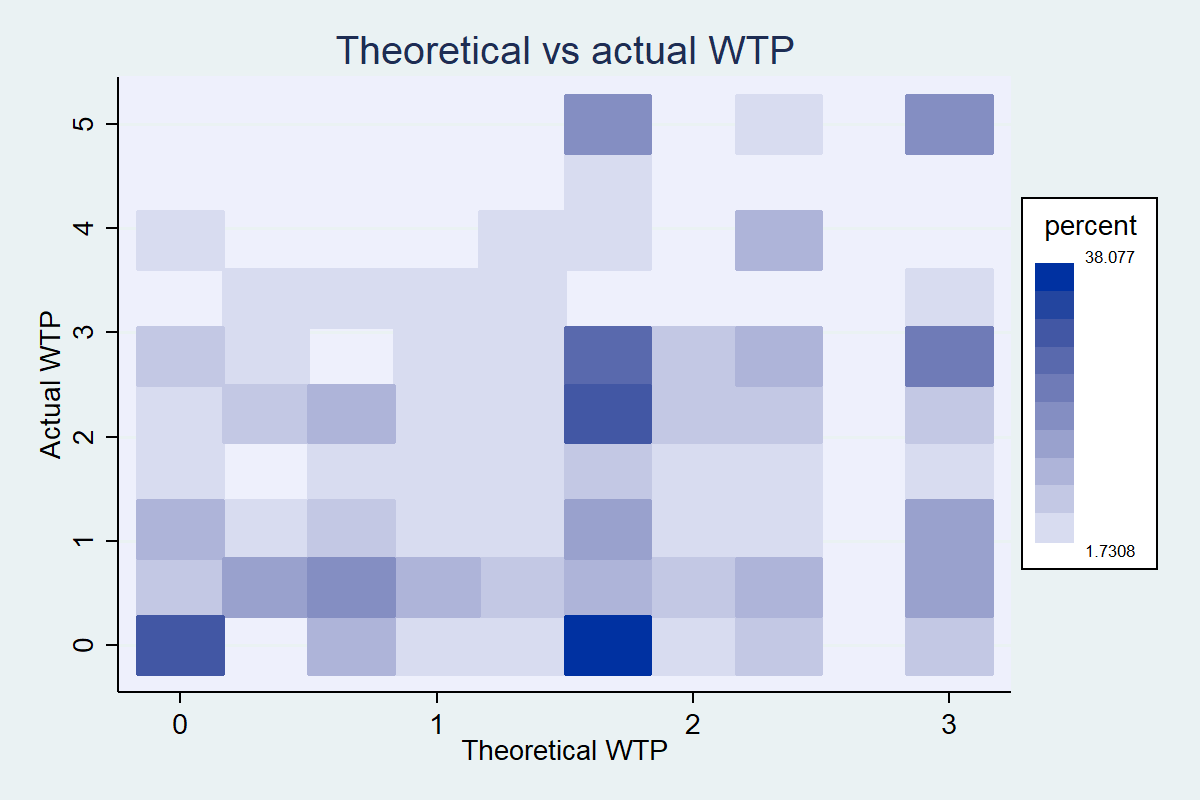
\includegraphics[scale=0.3]{Graphs/WTP_value_heat.png}
\end{figure}

\begin{figure}[H]
\centering
\caption{WTP discrepancy} \label{WTP_discrepancy_fig}

  \centering
  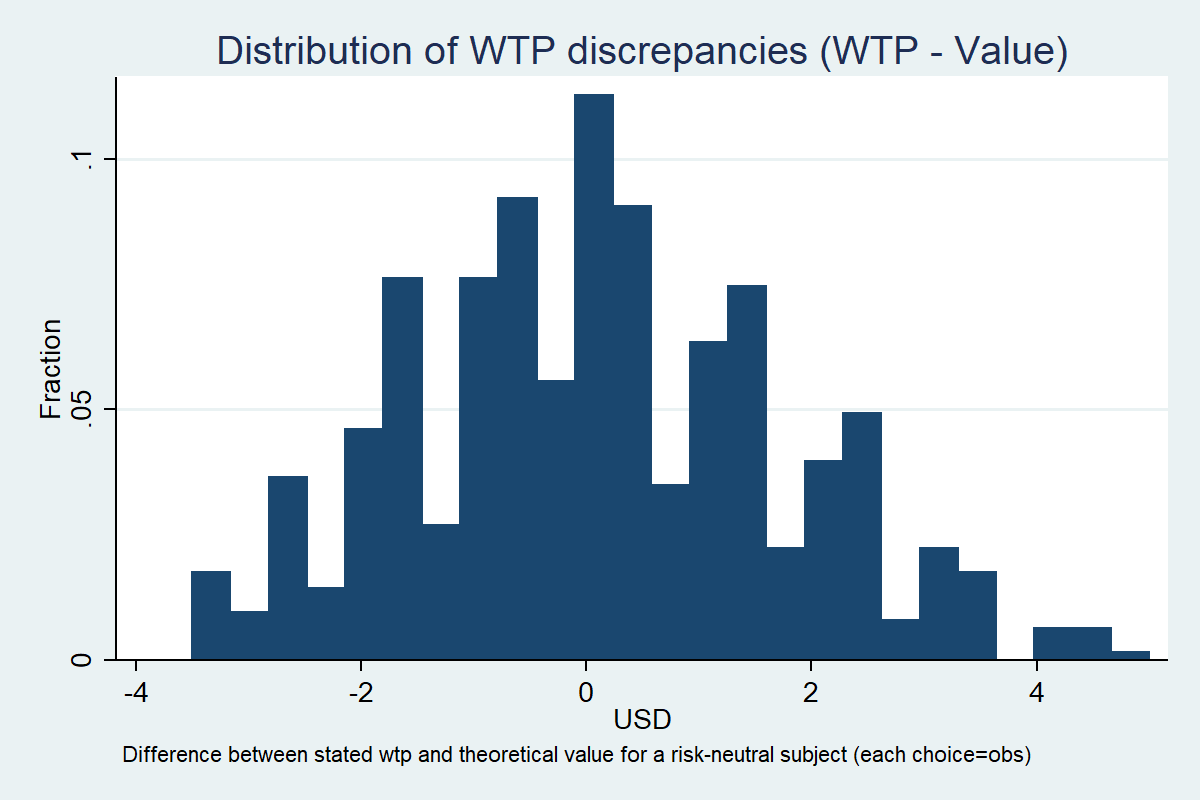
\includegraphics[scale=0.3]{Graphs/hist_WTP_discr1.png}

\end{figure}



\newpage
\section{Proofs}

\textbf{Proof of Proposition 1:} 
\begin{proof} If protection costs are low enough $c<\pi L$ than the risk-neutral decision-maker should always protect without a signal:
$$U=\max[\pi(Y-L)+(1-\pi)Y,Y-c]=Y-c$$

It means that a strictly risk-averse decision-maker with a utility function $u()$ should also protect:
$$\pi u(Y-L)+(1-\pi)u(Y)<u(\pi(Y-L)+(1-\pi)Y)=u(Y-c)$$

Then denote stochastic payoff with a signal as $X$ so that expected utility with a signal is $Eu(X-b)$ where $b$ is the willingness-to-pay solving:
$$Eu(X-b)=u(Y-c)$$
 Let $b_0$ be the willingness-to-pay for a risk-neutral decision-maker. By Jensen's inequality:
$$Eu(X-b_0)<u(EX-b_0)=u(Y-c)=Eu(X-b)$$

Because expected utility with a signal is a decreasing function of $b_0$ we obtain $b>b_0$. \end{proof}

\newpage
\section{Alternative Explanations}

We show that the observed pattern of switching sensitivities to false-positive and false-negative rates with priors is not consistent with the probability-weighting and preferences for certainty.  

\textbf{Loss-averse decision-maker.} A loss-averse decision-makers have extra-sensitivity to losses or deviations of incomes below a certain baseline. As a result, utility function becomes convex in the domain of losses. There are different functional specifications of loss aversion, but ---

\textbf{Probability-weighting decision-maker.} A decision-maker does probability weighting if it reacts to overreacts to very low probabilities and underreacts to very high probabilities. Their behavior can be described as a standard expected utility maximization but transforming all the probabilities to number closer to the middle of the support (1/2). We can show that probability weighting implies a reverse pattern of responses to false-positive and false-negative rates with priors and hence cannot explain our observations. Willingness-to-pay solves the following equation, which is equivalent to eqation () but with probabilities $x$ replaced by its monotonic transform $f(x)$:

\begin{equation}
\begin{split}
f(P(s=1))u(Y-b-c)+f(\pi P_{01})u(Y-b-L)+f((1-\pi)P_{00})u(Y-b)=\\=\max[u(Y-c),f(\pi) u(Y-L)+f((1-\pi)) u(Y)] 
\end{split}
\end{equation}

Taking derivatives from both sides we obtain:

 $${db\over dP_{10}}=-{(1-\pi)(u(Y-b)-u(Y-c-b))\over D(\pi, P_{01}, P_{10}, b)}$$
$${db\over dP_{01}}=-{\pi(u(Y-c-b)-u(Y-L-b))\over D(\pi, P_{01}, P_{10}, b)}$$


\textbf{Preferences for certainty.} \citet{eliaz_paying_2010} observe subjects paying for signals which have no potential effect on their decisions. Their theoretical explanation assumes that decision-maker's certainty in a chosen action directly affects their decision. In our setup it is equivalent to adding a strictly increasing function of the posterior belief $\mu$ to the consumption utility. Math ---

\end{document}